\documentclass{ociamthesis}
% \documentclass[12pt, oneside]{book}
\usepackage[utf8]{inputenc}
\usepackage[margin=3.5cm]{geometry}
\usepackage{listings}
\usepackage{tabularx}
\usepackage{rotating}
\usepackage{pdflscape}
\usepackage{setspace}
\usepackage{hyperref}
\usepackage{amsmath,amssymb,amsthm}
\usepackage{mathtools}
\usepackage{xcolor}
\usepackage{cleveref}
\usepackage{stmaryrd}
\usepackage{textcomp}
\usepackage{graphicx}
\usepackage{subfig}
\usepackage{subfig}
\usepackage[numbers]{natbib}
\usepackage{bm}
\usepackage[ruled]{algorithm}
\usepackage[noend]{algpseudocode}
\usepackage[colorinlistoftodos,prependcaption,textsize=tiny]{todonotes}
\usepackage{amartya_ltx}
\newtheorem{theorem}{Theorem}
\newtheorem{definition}{Definition}
\graphicspath{ {./images/} }

\title{Crafting Label Noise to Increase Adversarial Vulnerability in Deep
Learning Models}
\author{Candidate Number: 1048673}
\date{}
\college{}
\degree{MSc in Computer Science}
\degreedate{}

\doublespacing

\begin{document}
\maketitle

\chapter*{Acknowledgements}
Without the support and sacrifices of my mother, I could never have dreamt of
receiving an education. I would like to thank my supervisors, Professor Varun
Kanade, and Professor Philip Torr for their guidance throughout this project,
and also for access to the computational resources I required. I am grateful for
the interesting discussions I got to have with them throughout the summer. I am
grateful to Amartya Sanyal, for being a mentor for the project and my closest
friend. My year at Oxford, in the midst of a pandemic would have been very empty
without the warm group of friends at St Hugh's College. I am also thankful to my
course supervisor, Professor Bill Roscoe for being a guiding light, and for
priceless advice.

\chapter*{Abstract}
Deep Neural Networks have achieved the state of the art in many tasks. However,
recently there have been concerns regarding their robustness, and hence
reliability, when being deployed in mission critical applications. It seems that
Neural Networks can be easily fooled, by adding small perturbations to the
input. There has been a recent flow of literature in the direction of
purposefully making modifications to datasets in order to increase the
vulnerability of Neural Networks trained on them. Such modifications to datasets
with malicious intent, is called dataset poisoning.

Label flipping is one such dataset poisoning attack, where certain samples from
a dataset are chosen, and mislabeled on purpose. Surprisingly, Neural Networks
manage to generalise very well, even after memorising label noise. However,
their adversarial vulnerability takes a huge fall. In this thesis, we will study
the nature of decision boundaries learnt by networks as they memorise label
noise. Our attempt is to then utilise this knowledge to craft label noise, i.e.,
select points to flip in a dataset, in order to maximise the adversarial
vulnerability of networks trained on it. The number of points we can select to
label-flip is naturally constrained by a budget. 

Talk about results here. Further, a suprising experimental result we observed,
is that placing mislabeled points in the highest probability density regions of
the data distribution has minimal effect on the adversarial accuracy of a
network that memorises it. We also extend some previous theoretical results
regarding uniform label noise, with additional reasonable assumptions about
networks, such as Lipschitzness.

\tableofcontents

\chapter{Introduction}

\section{The Problem}

Deep Neural Networks (DNNs) have gained a lot of popularity in the Machine
Learning Community. The fact that they are universal approximators
\citep{hornik1989multilayer}, coupled with good training algorithms, and an
abundance of data and powerful hardware, are some factors that have contributed
to their popularity. These have helped deep learning achieve the state of the
art in many tasks, from computer vision \citep{imagenet}, to machine translation
\citep{seq2seq,attention-is-all-you-need}, to achieving superhuman performance
in board and computer games \citep{alpha-zero, starcraft}. However, the
reliability of neural networks is still in question. The work of \citet{42503}
opened up a new line of research on the robustness of neural networks. Neural
Networks seem to be sensitive to small perturbations in the input.

Recent works \citep{belkin2018understand,DBLP:journals/cacm/ZhangBHRV21} have
pointed out that several over-parameterized machine learning models can memorize
label noise (mislabelled points), which is surprisingly already present in
widely used datasets \citep{sanyal2021how} such as MNIST and CIFAR-10, without
showing a noticeable drop in their test accuracies. This has been investigated
with artificially induced label noise in standard datasets as well
\citep{sanyal2021how}, and is referred to as \emph{benign overfitting}.

However, memorizing noisy data does come with downsides. \citet{sanyal2021how}
investigated the consequences of memorizing \emph{uniform} label noise on the
adversarial error of the model. They showed that the adversarial error increases
in the presence of such label noise, because the model becomes increasingly
vulnerable in regions where a wrong label has been memorized. So, a model that
is trained on data with label noise might perform very well on unseen test data,
but it will be highly adversarially vulnerable, much more than what a model
trained on clean data would be. This means we, as attackers, can add human
imperceptible perturbations to the inputs of a network and get the network to
misclassify them.

While \citet{sanyal2021how} experimentally and theoretically investigated a
setting where models memorize \emph{uniform} label noise, there has not been any
study towards carefully \emph{crafting} label noise such that if it is
memorised, robustness is hurt massively. More precisely, the question we seek to
answer is: mislabeling which points in a dataset would cause a greater fall in
the adversarial vulnerability? The answer to this question could be used to
select points in a dataset which we could mislabel, and render a victim's model,
trained on this ``poisoned" data, to be highly adversarially vulnerable.

% rephrase this
The bound proven in Theorem 1 of \citet{sanyal2021how} makes no assumption
regarding the classifier that memorises a dataset with uniform label noise. The
worst case for high adversarial error is assumed, in order to arrive at the
bound: the case where mislabeled points get memorised discontinuously. In this
worst case, the classifier gets the highest possible test accuracy, getting the
wrong answer only at mislabeled points, and nowhere else. The bound naturally
follows from this. There exist $l_p$ balls of radius $\epsilon$ (the
attack radius) around mislabeled points within which all points are vulnerable.
In practice, networks learned with SGD are much smoother, and end up learning
regions around these mislabelled points where the network will produce the wrong
label, rather than just at the mislabelled points.

The problem at hand is in the following direction. Given a dataset, we are to
find out which points in the dataset can be label-flipped , so that a neural
network trained on the dataset becomes highly adversarially vulnerable while not
showing an appreciable drop in its test accuracy. The number of points we can
flip is constrained by a budget. Victims who might deploy their model trained on
such a poisoned dataset, will have vulnerabilities in their system. This study
is also in the hope that we can uncover some properties of neural networks
fitting mislabeled points, and observe the effects of memorizing label noise, so
that we might be able to come up with defences to the same.

When mislabeled points are introduced into the dataset, deep neural networks
trained on the dataset learn regions where they misclassify the input, and our
aim is to also study the nature of these regions. The experiments in this thesis
reveal whether these regions are seperate pockets, such that nearby points
become vulnerable, or are extensive regions which render regions far away from
the mislabeled training point vulnerable. 

\section{Contributions}
Our contributions in this thesis are threefold:
\begin{enumerate}
    \item Extending a previous theoretical result on benign overfitting, with
    added Lipschitzness assumptions on networks, in the context of uniform label
    noise.
    \item Showing that placing mislabeled points at the highest probability
    density regions does not hurt adversarial vulnerability, indicating that the
    proven theoretical bound in literature is vacuous in practice.
    \item Coming up with an experimental setup that helps identify points which
    are best to be mislabeled, for hurting the adversarial accuracy of a model
    trained on them. The experiments we did also indicate why randomly selecting
    points to label-flip in a popular dataset like MNIST is still very good.
    Points which massively hurt adversarial accuracy on being mislabeled turn
    out to be high in number. This also identifies a significant property of
    mislabeled points that causes such a massive drop in the adversarial
    accuracy: they draw and stretch the decision boundary, and this will be
    explained in detail in chapter \ref{chapter:experiments}. The selection of
    such points seems to be dependent on the dataset under study. While our
    final procedure is not a function into which we can simply plug in a dataset
    and receive a poisoned version, we do have an impactful toolset that guides
    the selection of training points to label-flip.
\end{enumerate}


\chapter{Background}
\section{The supervised classification problem}

Consider a distribution $\mathcal{P}: \mathbb{R}^d \to \mathbb{R}_{\geq_0}$ from
which datapoints are sampled, and a function $c: \mathbb{R}^d \to \Omega$,
called the \emph{ground truth} function. $\Omega$ is a discrete set of
\emph{classes} that instances from $\mathbb{R}^d$ need to be mapped into. Given
$n$ points sampled i.i.d. from $\mathcal{P}$, in a \emph{training set}
$D=\{\vec{x_i}\}_{i=1}^{n}$, the supervised classification problem is to find a
function with high probability, that classifies samples from $\mathcal{P}$
reliably as $c$ would have. This notion of reliability is captured formally
through the \emph{natural risk}, which we will define shortly.

The \emph{natural risk} $R_{\text{Nat}}(\mathcal{C}) $ of a classifier
$\mathcal{C}: \mathbb{R}^d \to \Omega$, is defined as

\begin{equation}
    R_{\text{Nat}}(\mathcal{C}) = \mathbb{P}_{\vec{x} \sim \mathcal{P}}
    [c(\vec{x}) \neq \mathcal{C}(\vec{x})] = \int_{\mathbb{R}^d} \mathcal{P}(\vec{x})
    \cdot\llbracket c(\vec{x}) \neq \mathcal{C}(\vec{x}) \rrbracket~\vec{dx}
\end{equation}

In other words, the natural risk is the probability of the classifier producing
the wrong answer. In practice, we carry out a Monte-Carlo estimation of the
natural risk, by finding the fraction of points in an unseen set of points
sampled i.i.d. from $\mathcal{P}$ (called the ``test set") for which the
classifier gets the incorrect output. This estimate is also called the ``test
error". Precisely, let this test set be denoted as $D_\text{test} =
\{(\vec{x_i}, y_i=c(\vec{x_i})) \}_{i=1}^m$. Then,
% sum
\begin{equation*}
    \hat{R}_{\text{Nat}}(\mathcal{C})
    = \frac{1}{|D_\text{test}|} \cdot \sum_{(\vec{x}, y) \in D_\text{test}} 
    \llbracket y \neq \mathcal{C}(\vec{x}) \rrbracket
\end{equation*}

$\mathcal{C}$ is a ``hard'' classifier in the discussion above. It produces one
class in its output. We will be dealing with \emph{probabilistic} classifiers as
well in the discussions, where $\mathcal{C}:\mathbb{R}^d\to\Delta^\Omega$
produces a probabity distribution over classes, where $\Delta^\Omega$ is the
$k$-dimensional simplex. In such a case, the final decision made by the
classifier will be $\underset{\Omega}{\arg\max}~\mathcal{C}(\vec{x})$. The
nature of the classifier under study will be clear from the context, and all
classifiers producing a distribution over the classes will be explicitly
referred to as probabilistic classifiers.

\section{Neural networks}

Deep Neural Networks are a family of over-parametrised models. They are proven
\emph{universal approximators} \citep{hornik1989multilayer}, which means with
enough parameters, they can approximate any function with arbitrarily small
error.

DNNs are composed of \emph{layers}, with each layer parameterized by
\emph{weights} and \emph{biases}. Each layer takes in a vector and produces
another vector. This is done by first doing an affine transformation of the
input vector, which is entirely specified by the weight matrix and bias of that
layer. This transformation yields a vector which is then passed through an
\emph{activation function}. DNNs acquire their non-linearity through these
activation functions. More precisely, let the $i$th layer of a network be
denoted as $L_i: \mathbb{R}^{d_{i}} \to \mathbb{R}^{d_{i+1}}$. Let its weight
matrix be $W_i \in \mathbb{R}^{d_i \times d_{i+1}}$, bias be $\vec{b}_i \in
\mathbb{R}^{d_{i+1}}$ and activation function be $\sigma$. Then the layer $L_i$
is defined as the following function:

\begin{equation*}
    L_i(\vec{x})
    = \sigma(W_i\vec{x} + \vec{b}_i)
\end{equation*}

Then the entire DNN is simply a composition of all of its layers. So a DNN
$\mathcal{C}: \mathbb{R}^{d_\text{in}} \to \mathbb{R}^{d_\text{out}}$ having $k$
layers $L_1,...,L_k$ is defined as:

\begin{equation*}
    \mathcal{C} = L_k \circ L_{k-1} ... \circ L_1
\end{equation*}
The series of computations we perform while finding the outputs of each layer
for a given input is called a \emph{forward pass}.

The ReLU activation function is the most popular one. It is defined as
\begin{equation*}
    \text{ReLU}(x) = 
    \left\{
        \begin{array}{ll}
            0 & \quad x \leq 0 \\
            x & \quad x > 0
        \end{array}
    \right.
\end{equation*}
Two other popular activation functions are the sigmoid and tanh activations
\begin{equation*}
    \text{sigmoid}(x)=\frac{1}{1+e^{-x}}
\end{equation*} and
\begin{equation*}
    \text{tanh}(x) = 2\cdot\sigma(x) - 1
\end{equation*}
The above definitions involve scalar inputs to these functions. We will overload
vector inputs for the activation functions defined above, such that each
dimension in the input vector is passed through the activation function
considered.

For classification problems, we require the network to output a probability
distribution over classes in $\Omega$. This is achieved by using the
\emph{softmax} activation function, defined as:

\begin{equation*}
    \text{softmax}: \mathbb{R}^k \to \Delta^k~;~
    \text{softmax}(\vec{x}) = \vec{x'} \text{ s.t. } 
    \vec{x'}_i = \frac{e^{\vec{x}_i}}{\sum_{j=1}^{d}e^{\vec{x}_j}}
\end{equation*}
where $\Delta^k$ refers to the $k$ dimensional simplex.

The softmax function is essentially a soft, smooth version of the one-hot-argmax
function, which returns a one-hot vector of same dimensionality, with a $1$ at
the index with the maximal value in a vector, and 0 elsewhere. The above
activation produces a probability distribution over the dimensions. Hence, in
networks used for classification problems, we generally augment the final layer,
having $|\Omega|$ dimensional outputs, with the softmax activation function.
$\Omega$ here is the set of classes the classifier has to map into.

% what is architecture?
The dimensionalities of each layer, activations, number of layers, etc. are
design choices, and these constitute the \emph{architecture} of the network. Any
such design choice, be it the number of layers or the activation functions used,
induces inductive biases. We assume that there exists a function that is a good
enough approximation of the function we want, in the family of functions we
search over, referred to as the \emph{hypothesis class}. For instance, the
hypothesis class could be the set of neural networks with different values for
their parameters, but having the same architecture. Now, we will need to search
over this family of functions with the same architecture for the ``best" one,
having certain values for its parameters, which is what the \emph{training
algorithm} does.


Convolutional Neural Networks (CNNs) are DNNs that perform very well on image
data \citep{imagenet,neco.1989.1.4.541}, by capturing spacial correlations in
images. All experiments on image datasets done in this thesis utilise CNNs.

\subsection{Training algorithms}
\label{section:sgd}
Gradient Descent is an optimisation technique that assumes a first order
approximation of the objective function. Given a function $f(\vec{x})$, which
needs to be \emph{minimised} over $\vec{x}$, gradient descent attempts to find a
minimum by iteratively updating the current best as:
\begin{equation*}
    \vec{x_{i+1}}
    = \vec{x_i} -
        \alpha \cdot \nabla_\vec{x} f(\vec{x}) \bigr \rvert _{\vec{x}=\vec{x_i}}
\end{equation*}
where $\alpha$ is a hyperparameter called the \emph{learning rate}. Hence,
gradient descent requires gradients of $f$ computed w.r.t $\vec{x}$.

In machine learning, we might frequently require optimising over functions of
the form $\frac{1}{m}\sum_{i=1}^m g_i(\vec{x})$. Often, each term of this sum is
the contribution of each individual point in the dataset to the objective. This
requires gradient descent to evaluate
\begin{equation*}
    \nabla_\vec{x} \frac{1}{m}\sum_{i=1}^m \mathcal{L}_i(\vec{x})
    = \frac{1}{m} \sum_{i=1}^m \nabla_\vec{x} \mathcal{L}_i(\vec{x})
\end{equation*}
This is usually computationally expensive to evaluate, since one gradient
descent step will require computing gradients for each term, which frequently
evaluates to computing average gradients over the entire training set.
Stochastic Gradient Descent (SGD) involves sampling a small batch of samples
from the training set, and executing a gradient descent step using the mean
gradients for that batch, rather than the entire training set.

There are many other first-order gradient based optimizers, the most popular one
being the Adam optimizer \citep{Adam}. Adam has much higher convergence rates in
practice, compared to vanilla SGD. In all of the experiments in this thesis,
Adam is the optimizier used. % fix this

\subsection{Loss functions}
% remove "good"
% tweak the parameters - that is what optimisation is
To train networks, we need to have a metric that captures how ``good" a network
is. We could then optimise over this metric, and tweak the parameters of the
model hoping that the resultant model will have a low natural risk. Such metrics
are called loss functions.

For classification problems in this thesis, we will be using the \emph{Cross
Entropy Loss}, which is standard for neural network classifiers. For a ``target"
distribution $P$, and a distribution $Q$ both over a set $\Omega$, the
cross-entropy $H$ between $P$ and $Q$ has the lowest value when $P=Q$, and high
values when $Q$ is very different from $P$.
\begin{equation*}
    H[Q, P] = -\sum_{\omega \in \Omega} P(\omega) \log Q(\omega)
\end{equation*}

% fix phrasing here
% use one-hot function here
Given an input example $\vec{x}$, labeled with $y=c(\vec{x})$, a probabilistic
classifier $\mathcal{C}: \mathbb{R}^d \to \Delta^\Omega$ produces a distribution
over the set of classes ($\Omega$). The cross-entropy loss for this classifier
at the given datapoint $(\vec{x}, y)$ evaluates to
$H[\mathcal{C(\mathcal{\vec{x}})}, \vec{y}]$ where $\vec{y} \in \Delta^\Omega,
\vec{y}_j=\llbracket j == y \rrbracket$. $\Delta^\Omega$ refers to the
$k$-dimensional simplex.

\subsection{Backpropagation}
To train a neural network $\mathcal{C}$ with the algorithms mentioned in the
section \ref{section:sgd}, we require to compute $\mathbb{E}_{\vec{x} \sim
\mathcal{P}}[\nabla_\theta \mathcal{L}(\mathcal{C(\vec{x})}, c(\vec{x}))]$ where
$\mathcal{P}$ is the data distribution. In practice, this is done by sampling a
batch of $b$ samples $X=[\vec{x_i}\mid i \in [1..b]]$ uniformly from the test
set, and computing $\frac{1}{b} \sum_{i=1}^{i=b} \nabla_\theta
\mathcal{L}(\mathcal{C(\vec{x_i})}, c(\vec{x_i}))$.

In order to do this computation in neural networks, we require to methodically
apply the chain rule. The backpropagation algorithm does this. We first record
all computations we do during the forward pass, and the following recursive
relation is utilised to find the gradients of the loss with respect to one value
in this forward pass. Let this value be $v$, and all values dependent on $v$ be
$u_1... u_k$. Let $L$ denote the final value whose gradient we are to compute,
w.r.t. $v$, assuming we already have $\frac{\partial L}{\partial u_1}...
\frac{\partial L}{\partial u_k}$ and we know how to compute $\frac{\partial
v}{\partial u_i}$. Then,
\begin{equation*}
    \frac{\partial L}{\partial v} = \sum_{i=1}^k {\frac{\partial
v}{\partial u_i}\cdot \frac{\partial L}{\partial u_i}}
\end{equation*}

So we start from $\frac{\partial \mathcal{L}}{\partial \mathcal{L}}=1$, and work
``backwards" from there to compute all gradients, where $\mathcal{L}$ is the
loss.

The relation above can be applied to any network such that for each operation,
we can compute gradients of the operation's outputs w.r.t. its inputs, and
allows for far more flexibility than than just working for the model
architectures we discussed.

\section{Adversarial risk}

\citet{42503} discovered a significant property of deep neural networks: they
are sensitive to changes in the input. Networks trained on data drawn from a
distribution perform very well on unseen data from the same distribution, for
example that of handwritten digits, but are extremely sensitive to small, almost
human imperceptible input perturbations. This is generally referred to in
literature as \emph{Adversarial Vulnerability}.
\citet{Goodfellow2015ExplainingAH} and \citet{madry2019deep} showed some methods
to craft such perturbations, and these are called \emph{adversarial attacks}.
These attacks will be discussed later, in \cref{section:standard-attacks}.

This sensitivity to input perturbations is a significant vulnerability, since
the changes in the input can be imperceptible to humans. Deep Learning models,
with their improving real-world performance
\citep{imagenet,imagenet-superhuman}, are begining to get deployed in mission
critical systems \citep{adv-vuln-in-mission-critical}, and such vulnerabilities
raise questions about the reliability of neural networks for such applications.

The adversarial vulnerability of a classifier $\mathcal{C}$ is quantified
through the \emph{adversarial risk}. While there are a multitude of ways in
literature in which adversarial vulnerability has been defined, we are concerned
with adversarial vulnerability in the context of $l_p$ perturbations. The
adversarial risk $R_{\text{Adv}}^{\rho}(\mathcal{C}) $ of a classifier
$\mathcal{C}: \mathbb{R}^d \to \Omega$ in a classification problem where
datapoints are drawn from the distribution $\mathcal{P}: \mathbb{R}^d \to
\mathbb{R}_{\geq 0}$ where $d$ is the data dimensionality, and ground truth
labeling function $c: \mathbb{R}^d \to \Omega$, where $\Omega$ is the set of
classes, is defined as

\begin{equation} \label{eq:adv-risk}
    \begin{split}
    R_{\text{Adv}}^{\rho}(\mathcal{C}) & = \mathbb{P}_{\vec{x} \sim \mathcal{P}}
    [\exists \vec{\tilde{x}} \in \mathcal{B}_\rho^p(\vec{x})~\text{s.t.}~c(\vec{x}) \neq \mathcal{C}(\vec{\tilde{x}})] \\
    & = \int_{\mathbb{R}^d} \mathcal{P}(\vec{x})
    ~\llbracket \exists \vec{\tilde{x}} \in \mathcal{B}_\rho^p(\vec{x})~\text{s.t.}~c(\vec{x}) \neq \mathcal{C}(\vec{\tilde{x}}) \rrbracket~\vec{dx}
    \end{split}
\end{equation}

where $\mathcal{B}_\rho^p(\vec{x})$ is the set of all points inside an $l_p$
ball around $\vec{x}$, given by 

\begin{equation*}
    \mathcal{B}_\rho^p(\vec{x}) = \{\vec{x'} \in
    \mathbb{R}^d \mid \rho \geq \norm{\vec{x'} - \vec{x}}_p\}
\end{equation*}
for some norm $p$.

The adversarial risk intuitively captures the probability that we get an input
$\vec{x}$ such that it can be perturbed, so that the classifier gives an output
that $\vec{x}$ was not labeled with. Further, this perturbation has to be within
a constrained region. This definition attempts to formalise the notion of
``imperceptibility'' of such attacks, through the $l_p$-ball constraint. In
practice, this risk is estimated by utilizing some standard attack strategy to
calculate perturbations, such as those explained in
\cref{section:standard-attacks}. We then find the fraction of test-set points
for which the attack strategy could successfully find a perturbation that could
make the classifier misclassify. This fraction gives the \emph{adversarial
error} of the classifier, an estimation of the adversarial risk. The
\emph{adversarial accuracy} of the classifier is the fraction of test-set points
for which the attack strategy could not find a perturbation that gets the
classifier to misclassify.


Given a probabilistic classifier $\mathcal{C}: \mathbb{R}\to\Delta^\Omega$ and a
point $\vec{x} \sim \mathcal{P}$, the problem of finding an adversarial example
for $\vec{x}$, i.e. finding an $\vec{\tilde{x}} \in
\mathcal{B}_\rho^p(\vec{x})~\text{s.t.}~c(\vec{x}) \neq
\mathcal{C}(\vec{\tilde{x}})$ can be written as a constrained optimization
problem:

\begin{equation*}
    \vec{\tilde{x}} = \underset{\vec{u} \in \mathcal{B}_\rho^p(\vec{x})}
    {\arg\max}~\mathcal{L}(\mathcal{C}(\vec{u}), c(\vec{x}))
\end{equation*}
where $\mathcal{L}$ is a loss function, and could be the same loss function used
to train the model. So we maximize this loss inside the $l_p$ ball around
$\vec{x}$ to find an adversarial example. The solution to the above optimisation
problem is an \emph{untargeted} adversarial example. This means that the
resultant adversarial example could be classified by the model as any wrong
class, which is why we call algorithms that solve or approximate the above as
\emph{untargeted attacks}.

We could also have \emph{targeted attacks}, which provide greater control to
attackers. Targeted attacks involve creating adversarial examples such that the
classifier classifies it to be of a particular \emph{target class}. Let the
target class be $t$. Then the constrained optimisation problem for a targeted
attack around $\vec{x}$ is

\begin{equation*}
    \vec{\tilde{x}_t} = \underset{\vec{u} \in \mathcal{B}_\rho^p(\vec{x})}
    {\arg\min}~\mathcal{L}(\mathcal{C}(\vec{u}), t)
\end{equation*}


The brief review on attack strategies that follows this discussion is based on
different ways to go about computationally solving the above optimisation
problems.



\begin{figure}[!h]
    \centering
    % 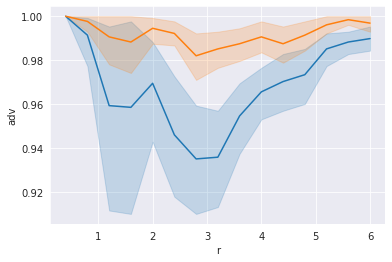
\includegraphics[scale=0.75]{normal_training_toy_dataset}
    \subfloat[][Classified as a ``5"]{{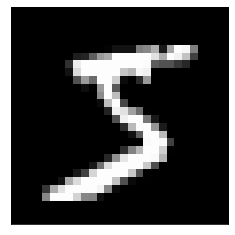
\includegraphics[scale=0.35]{clean-5.png}}}
    \qquad
    \subfloat[][Classified as a ``3"]
    {{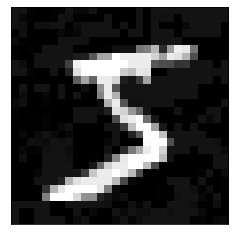
\includegraphics[scale=0.35]{perturbed-5-classified-3.png}}} \caption{A
    convolutional neural network trained on the MNIST dataset, attained 99.19\%
    test accuracy. The classifier predicts the image of ``5" on the left
    correctly with 100\% confidence. The same ``5" was perturbed, within a
    $0.04~l_\infty$ radius of the original ``5". The same classifier classifies
    this ``5" as a ``3", with more than 60\% confidence. This classifier has 0\%
    adversarial accuracy for a $0.3~l_\infty$ radius, which means for each point
    in the test set, we can find a small enough perturbation to add to the
    original image, and get the classifier to misclassify. The reader might need
    to view the page from different angles to perceive the difference between
    the two images.}
    \label{fig:adversarial-example-5}
\end{figure}

\section{Standard attacks for neural networks in literature}
\label{section:standard-attacks}

Here, we discuss 2 popular attack techniques in literature. When we use the term
\emph{attack}, the problem we attempt to solve is finding an adversarial
example, i.e., given a point from the data distribution, we are to find out a
point within an $l_p$ ball (of some radius $\rho$) around that point, such that
the model gives the wrong output for that point. For a \emph{targeted attack},
given a point $\vec{x}$ with label $c(\vec{x})$ from the data distribution, we
are to find a point $\vec{x'}$ inside an $l_p$ ball of certain radius around
$\vec{x}$, such that the model classifies $\vec{x'}$ as a target class $t$.

Reiterating, our objective will be to solve a constrained optimisation problem,
minimising or maximising the loss, depending on whether or not we are doing a
targeted, or untargeted attack.

Let $\mathcal{L}: \Gamma(\Omega) \times \Omega \to \mathbb{R}$ be the loss
function considered, where $\Omega$ is the set of classes and $\Gamma(\Omega)$
is the set of all probability distributions over $\Omega$. For our discussion,
it does not matter which loss is used, as long as it penalizes, or has high
values when the model produces the wrong class prediction, and low value when it
gives the right one. The cross entropy loss is the most popular choice. Given a
data-point $\vec{x}$ and neural network classifier $\mathcal{C}_\vec{\theta}$
(modelling a probabilistic classifier) parameterized by $\vec{\theta}$, these
methods rely on computing the loss value by forward propagating through
$\mathcal{C}_\vec{\theta}$, and then backpropagating, computing gradients all
the way to the inputs, finding the gradient of the loss with respect to the
input.

Essentially, we compute the following:
\begin{equation*}
    \vec{\Delta x}
    = \vec{\nabla}_\vec{p} \mathcal{L}(\mathcal{C}_\theta (\vec{p}), y)
    \bigr \rvert_{\vec{p}=\vec{x}}
\end{equation*}

We use the above computed value to carry out gradient ascent on the input for
untargeted attacks, and gradient descent on the same for targeted attacks,
setting $y=t$ where $t$ is the target class. Since we require access to the
model and all the computations done by it to compute the gradient above, these
attacks are also referred to as \emph{white box gradient based attacks}. There
exist \emph{black box} \citep{simba,genattack,prior-conv} attacks as well, where
access to, or knowledge about the model is restricted. These black box attacks
are however, out of the scope of our discussion.

\subsection{Fast Gradient Sign Method}
The Fast Gradient Sign Method (FGSM) \citep{Goodfellow2015ExplainingAH}, is a
one step procedure, and requires only one forward-backward pass through the
network. The constraint assumed for the attack is $\epsilon$ radius in
$l_\infty$ norm, which allows the attacker to produce adversarial examples for
$\vec{x}$ within an $\epsilon$ radius $l_\infty$ ball around $\vec{x}$. The
adversarial example produced by FGSM is given by:
\begin{equation*}
    \vec{x'}
    = \vec{x} + \epsilon \cdot
    \text{sign}(\vec{\nabla}_\vec{p} \mathcal{L}(\mathcal{C}_\theta (\vec{p}), y)
    \bigr \rvert_{\vec{p}=\vec{x}})
\end{equation*}
for an untargeted attack, and
\begin{equation*}
    \vec{x'}
    = \vec{x} - \epsilon \cdot
    \text{sign}(\vec{\nabla}_\vec{p} \mathcal{L}(\mathcal{C}_\theta (\vec{p}), t)
    \bigr \rvert_{\vec{p}=\vec{x}})
\end{equation*}
for a targeted attack. The sign function is:
\begin{equation*}
    \text{sign}(x) = 
    \left\{
        \begin{array}{ll}
            0 & \quad x = 0 \\
            \frac{x}{|x|} & \quad x \neq 0
        \end{array}
    \right.
\end{equation*}
and the above function is overloaded to vectors as an elementwise operation. The
sign of gradients, scaled by $\epsilon$ are used for updates to ensure that the
steps taken are small.


\subsection{Projected Gradient Descent}
The Projected Gradient Descent (PGD) \citep{madry2019deep} attack is the most
popular adversarial attack in literature. Throughout this thesis, wherever we
refer to attacks in experiments, we refer to PGD attacks. Popularly in
literature, and in this thesis as well, whenever the adversarial accuracy of a
network has to be evaluated, we iterate through the test set, and find out the
fraction of the test set for which the PGD attack was unsuccessful.

The PGD attack requires the following arguments and hyperparameters:

\begin{enumerate}
    \item Attack-steps $m$: This is the number of iterations the PGD algorithm
    is going to take.
    \item Step-size $\mu$: This is the size of each update the algorithm will
    take. The impact of this hyperparameter will be shown in the update equation
    below.
    \item Attack-norm $p$: Perturbations are constrained to be within a region
    around the input $\vec{x}$. This distance constraint is in the form of a
    norm, which we will call the \emph{attack-norm}. For instance, perturbations
    could be constrained within an $l_\infty$ ball $(p=\infty)$ of the input.
    \item Attack-radius $\epsilon$: This is the radius of the $l_p$ ball within
    which the perturbed image should lie around the original image.
\end{enumerate}
We repreatedly perturb the current perturbed image using FGSM, and project it
back onto the $l_p$ ball around the original input. Using the PGD algorithm with
attack norm $p$ is generally also referred to as ``using an $l_\infty$
PGD-adversary. The PGD algorithm is as shown in algorithm
\ref{algorithm:untargeted-pgd}.

\begin{algorithm}[!h]
\caption{Projected Gradient Descent}
\begin{algorithmic}[1]
\Procedure{Targeted-PGD}{$\mathcal{C}_\theta, \vec{x}, t, \epsilon, p, m, \mu$}
    \State $\vec{x_0} \gets \vec{x}$
    \For{$i \gets [1..m]$}
        \State $\vec{x_i} \gets$ \textproc{Targeted-FGSM}($\mathcal{C}_\theta, \vec{x_{i-1}}, t, \mu$)
        \State $\vec{x_i} \gets$ \textproc{Project}($\vec{x_i}, \mathcal{B}_\rho^p(\vec{x})$)
                \Comment{Project onto $l_p$ ball around $\vec{x}$}
    \EndFor
    \State \Return $\vec{x_m}$
    \label{algorithm:targeted-pgd}
\EndProcedure
\\
\Procedure{Untargeted-PGD}{$\mathcal{C}_\theta, \vec{x}, y, \epsilon, p, m, \mu$}
    \State $\vec{x_0} \gets \vec{x}$
    \For{$i \gets [1..m]$}
        \State $\vec{x_i} \gets$ \textproc{Untargeted-FGSM}($\mathcal{C}_\theta, \vec{x_{i-1}}, y, \mu$)
        \State $\vec{x_i} \gets$ \textproc{Project}($\vec{x_i}, \mathcal{B}_\rho^p(\vec{x})$)
                \Comment{Project onto $l_p$ ball around $\vec{x}$}
    \EndFor
    \State \Return $\vec{x_m}$
    \label{algorithm:untargeted-pgd}
\EndProcedure
\\
\Procedure{Targeted-FGSM}{$\mathcal{C}_\theta, \vec{x}, t, \epsilon$}
    \State $d \gets \mathcal{C}_\theta(\vec{x})$ 
            \Comment{Forward pass. $d \in \Gamma(\Omega)$ is the network's output}
    \State $\ell \gets \mathcal{L}(d, t)$
            \Comment{Operations are recorded to support backward-pass}
    \State $\vec{\Delta x}\gets\vec{\nabla}_\vec{p} \mathcal{L}(\mathcal{C}_\theta (\vec{p}), t)
    \bigr \rvert_{\vec{p}=\vec{x}}$
            \Comment{Backpropagate}
    \State $\vec{x'}\gets\vec{x} - \epsilon \cdot \text{sign}(\vec{\Delta x})$
    \State \Return $\vec{x'}$
    \label{algorithm:targeted-fgsm}
\EndProcedure
\\
\Procedure{Untargeted-FGSM}{$\mathcal{C}_\theta, \vec{x}, y, \epsilon$}
    \State $d \gets \mathcal{C}_\theta(\vec{x})$ 
            \Comment{Forward pass. $d \in \Gamma(\Omega)$ is the network's output}
    \State $\ell \gets \mathcal{L}(d, t)$
            \Comment{Operations are recorded to support backward-pass}
    \State $\vec{\Delta x}=\vec{\nabla}_\vec{p} \mathcal{L}(\mathcal{C}_\theta (\vec{p}), y)
    \bigr \rvert_{\vec{p}=\vec{x}}$
            \Comment{Backpropagate}
    \State $\vec{x'}\gets\vec{x} + \epsilon \cdot \text{sign}(\vec{\Delta x})$
    \State \Return $\vec{x'}$
    \label{algorithm:untargeted-fgsm}
\EndProcedure\

\end{algorithmic}
\end{algorithm}



% \subsection{Adversarial Training}
% This is a 


\section{Benign Overfitting and label noise}
\label{section:benign}
As showed by \citet{DBLP:journals/cacm/ZhangBHRV21}, networks show respectable
generalisation error even after memorising training data that has high levels of
label noise. This phenomenon of DNNs is referred to in literature as
\emph{benign-overfitting}. \citet{bartlett2020benign} study this phenomenon in
the context of linear regression problems.

\citet{sanyal2021how} showed that while benign overfitting does not
significantly harm the natural accuracy of classifiers, it massively harms the
adversarial accuracies of the same models, studying the problem mainly in the
context of uniform label noise. All experiments in this thesis are consistent
with the same: classifiers trained on noisy data have high natural accuracy but
low adversarial accuracies.

A significant theoretical result shown by \citet{sanyal2021how} is the
following:

\begin{theorem}
    \label{theorem:how-benign-bo}
    Let $\mathcal{C}$ be a classifier, and $\mathcal{D}: \mathbb{R}^d \to
    \mathbb{R}_{\geq 0}$ the data distribution, and $c: \mathbb{R}^d \to \Omega$
    be the ground truth labeling function, where $\Omega$ is the set of classes.
    If there exist constants $c_1 \geq c_2 > 0, \rho > 0$ and a set $\zeta
    \subset \mathbb{R}^d$, such that
    \begin{enumerate}
        \item $\mathbb{P}_{\vec{x} \sim \mathcal{D}} \bigg [~\underset{\vec{s}
        \in \zeta}{\bigcup}~\mathcal{B}_\rho^p(\vec{s}) \bigg ] \geq c_1$
        \item $\forall \vec{s} \in \zeta,~~ \mathbb{P}_{\vec{x} \sim
        \mathcal{D}} [\mathcal{B}_\rho^p(\vec{s})] \geq \frac{c_2}{|\zeta|}$
        \item $\forall \vec{s} \in \zeta,~\forall \vec{u}, \vec{v} \in
        \mathcal{B}_\rho^p(\vec{s}),~c(\vec{u}) = c(\vec{v})$
    \end{enumerate}
    where $\mathcal{B}^p_\rho(\vec{x})$ is a $\rho$-radius $l_p$ ball around
    $\vec{x}$. Let S be a training set, obtained by taking $n$ i.i.d. samples
    from $\mathcal{P}$, and labeling each with $c(.)$ with $\eta$ probability,
    or some incorrect class with probability $1-\eta$. Let $\mathcal{C}$ be a
    classifier such that it has a 100\% training accuracy on $S$. This means it
    gets the correct class on unflipped points, and has also memorized the wrong
    label on flipped points. Then, if $n \geq \frac{|\zeta|}{\eta c_2} \log
    (|\zeta|/\delta)$, with at least $1-\delta$ probability,
    $\mathcal{R}_{\text{Adv}}^{2\rho}(\mathcal{C}) \geq c_1$.
\end{theorem}

Theorem \ref{theorem:how-benign-bo} establishes that if the data distribution
has regions of high probability density, then a classifier trained on data
sampled from that distribution, injected with uniform label noise will have high
adversarial error, with high probability. Secondly, the result does not require
any assumption regarding the classifier. $\mathcal{C}$ could be a
1-nearest-neighbour classifier or a massive neural network, as long as it
memorises the entire training set. The adversarial risk in the bound comes from
the nearby probability mass, around mislabeled training points.


This result inspired the first few algorithms we tried out, which were based on
the idea that placing mislabeled points at the highest probability density
regions might be optimal to harm the adversarial accuracy of models trained on
the data. This is for the case where there is no uniform label noise. Rather, we
as attackers, are allowed to change the labels of a few points in the dataset.


\section{Dataset poisoning}
\emph{Dataset poisoning} \citep{just-how-toxic,
DBLP:journals/corr/abs-1712-05526} is a general term referring to the
manipulation of a dataset by an agent, in order to cause vulnerabilities in any
system that relies on this data. Modifications could be adding new malicious
samples, changing existing samples, or perhaps changing labels.

Backdoor attacks
\citep{DBLP:journals/corr/abs-1712-05526,hidden-trigger-backdoor,transferable-clean-label-poisoning}
are popular dataset poisoning attacks which involve crafting and placing
data-points such that if a neural network classifier ends up memorising this
point, it will have certain regions that are adversarially vulnerable. The name
``backdoor" comes from the fact that samples that would seem to be of class $A$
to us humans, will be memorised by the classifier to be of class $B$, creating a
region (a ``backdoor") where we as attackers, can later query inputs (these
inputs may be adversarial examples) of one class, while the classifier predicts
those inputs to be of another class.

Label flipping attacks \citep{label-flip-SVMs,certified-robustness} are
poisoning attacks where we as attackers can change the labels of points in the
dataset. For example, we might flip malicious emails and label them as spam in
an email dataset, and any spam detection network that learns from this dataset
will have poor accuracy (natural or adversarial, depending on the attack), at
least for a subset of possible emails, which we can later use to our advantage
when the model gets deployed.

Dataset poisoning attacks constitute a relevant problem. This is because most
practical machine learning systems utilise data that is scraped, or curated by
another party. For the former case, we can craft malicious data-points, and
upload them online, waiting for someone to scrap it off and train their networks
on it \citep{transferable-clean-label-poisoning}. For the latter case, the
opportunity to inject malicious data-points into the dataset is more
straightforward. Unfortunately, we might not always be able to refrain from
using data from untrusted sources. Studying these attacks has the end-goal that
we could eventually device training schemes that produce classifiers that are
robust to these poisoning attacks.

The objective of this thesis is to study how label-flipping attacks can be
crafted to maximise the adversarial error of networks trained on poisoned data.
From this point onward, points in the dataset that we mislabel, will be refered
to as \emph{poisons}, \emph{flipped} points, or simply as \emph{mislabeled}
points.


\chapter{Is Lipschitzness always beneficial for robustness?}
\label{section:Lipschitzness-assumption}

\citet{sanyal2021how} showed a theoretical result regarding \emph{uniform} label
noise, stated above in \cref{section:benign}. The result signifies that when
uniform label noise is injected, if there are $l_p$ balls of high probability
mass with radius $\rho$, then with large enough number of samples, the
adversarial risk (attack radius and norm being $2\rho$ and $p$ respectively)
will be high with high probability. In order to bound the adversarial risk, the
worst case had to be assumed, where the classifier fits the dataset such that it
gets the wrong answer only at the mislabeled points, and the right answer for
every other input. This classifier will have the lowest possible natural risk.
Neural networks are practically smooth, and do not fit mislabeled points
discontinuously. Each mislabeled training point will hence have a region around
it, where the network produces the wrong answer. This is illustrated in
\cref{fig:dictionary}.

In this chapter, we develop theoretical and experimental results with
Lipschitzness assumptions. The results are classifier agnostic, but the
classifier must be Lipschitz.

\begin{figure}
    \centering
    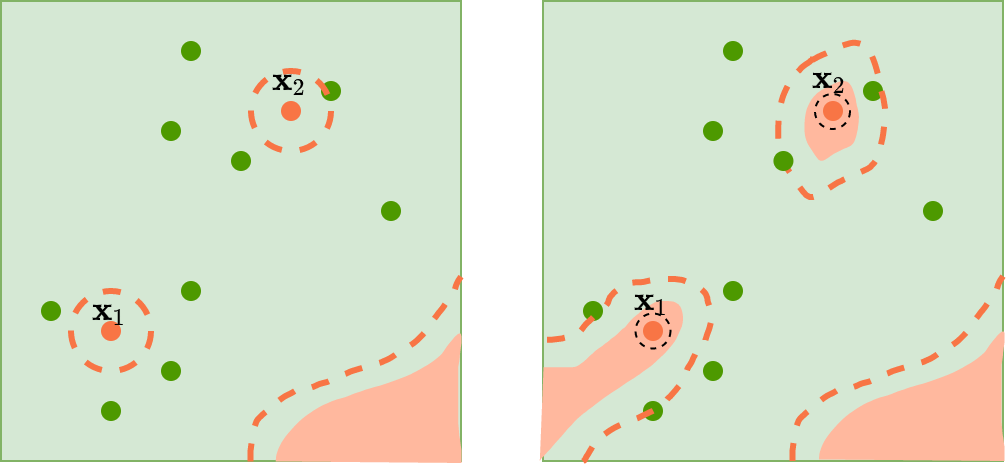
\includegraphics[scale=0.3]{memorizing-as-dictionary}
    \caption{The figure on the left shows a classifier learning mislabaled
    points as a dictionary, discontinuously. The figure on the right shows a
    classifier that is smooth around each training point. The dotted black
    circles indicate the smoothness guarantee. The radius of these circles is
    the distance that the input has to be changed by, in $l_2$ norm, for the
    classifier to change its output. The red dotted lines enclose regions which
    are adversarially vulnerable to being misclassfied from ``green'' to
    ``red'', under an $l_2$-norm attack regime of certain radius $\rho$. $\rho$
    is the margin between solid red regions and dotted red lines in the above
    figure.}
    \label{fig:dictionary}
\end{figure}

\begin{figure}
    \centering

\end{figure}

A function $f: X \to Y$ is $\kappa$-Lipschitz if there exists a constant
$\kappa$ s.t. $\forall \vec{x_1}, \vec{x_2} \in X$,
\begin{equation*}
    \label{eq:Lipschitz}
    \frac{d_1({f(\vec{x_1}), f(\vec{x_2})})}
        {d_2({\vec{x_1}, \vec{x_2}})}
    \leq \kappa
\end{equation*}
for some distance metrics $d_1, d_2$.

If the classifier under study is known to be Lipschitz continuous, including
this in Theorem-1 by \citet{sanyal2021how}, gives the same bounds for a weaker
adversary, i.e., we require a smaller attack-radius to get the same lower bound
on the adversarial risk.

\section{Improved bound with Lipschitzness Assumptions}

\begin{theorem}
    \label{theorem:Lipschitzness-extension}
    Let $\mathcal{C}: \mathbb{R}^d \to \Delta^\Omega$ be a probabilistic
    classifier and $\mathcal{C}_\text{hard}(\vec{x}) =
    \underset{\Omega}{\arg\max}~\mathcal{C}(\vec{x})$. Let $\mathcal{D}:
    \mathbb{R}^d \to \mathbb{R}_{\geq 0}$ be the data distribution, and $c:
    \mathbb{R}^d \to \Omega$ be the ground truth labeling function. $\Omega$ is
    the set of classes. If there exist constants $c_1 \geq c_2 > 0, \rho > 0$
    and a set $\zeta \subset \mathbb{R}^d$, such that
    \begin{enumerate}
        \item $\mathbb{P}_{\vec{x} \sim \mathcal{D}} \bigg [~\underset{\vec{s}
        \in \zeta}{\bigcup}~\mathcal{B}_\rho^p(\vec{s}) \bigg ] \geq c_1$
        \item $\forall \vec{s} \in \zeta,~~ \mathbb{P}_{\vec{x} \sim
        \mathcal{D}} [\mathcal{B}_\rho^p(\vec{s})] \geq \frac{c_2}{|\zeta|}$
        \item $\forall \vec{s} \in \zeta,~\forall \vec{u}, \vec{v} \in
        \mathcal{B}_\rho^p(\vec{s}),~c(\vec{u}) = c(\vec{v})$
    \end{enumerate}
    where $\mathcal{B}^p_\rho(\vec{x})$ is a $\rho$-radius $l_p$ ball around
    $\vec{x}$. Let $S=\{(\vec{x_i},y_i)\}_{i=1}^n$ be a training set, obtained
    by taking $n$ i.i.d. samples from $\mathcal{P}$, and labeling each sample
    $\vec{x_i}$ with $y_i=c(\vec{x_i})$ with $\eta$ probability, or any class
    $y_i\in\Omega\setminus\{c(\vec{x_i})\}$ with $1-\eta$ probability.
    
    If $\mathcal{C}$ is such that 
    \begin{enumerate}
        \item $\mathcal{C}_\text{hard}$ has 100\% training accuracy on $S$, and
        $\mathcal{C}$ has a margin \footnote{The margin here refers to the
        difference between the highest and second highest probabilities in the
        classifier's output.} of $\chi$ on the training set points.
        \item $\mathcal{C}$ is locally Lipschitz, such that $~\forall \vec{u},
        \vec{v} \in \mathbb{R}^d$,
            \begin{equation*}
                \frac{\norm{\mathcal{C}(\vec{u}) - \mathcal{C}(\vec{v})
                }_\text{TV}}
                    {\norm{\vec{u} - \vec{v}}_p} 
                \leq \kappa
            \end{equation*}
    \end{enumerate}
    where the total variation distance $\norm{p-q}_\text{TV}$ between two
    distributions $p$ and $q$ on a finite set $\Omega$ is given by
    \begin{equation*}
        \norm{p-q}_\text{TV} = \frac{1}{2}\sum_{\omega\in\Omega} 
        |p(\omega)-q(\omega)|
    \end{equation*}
    
    Then, if $n \geq \frac{|\zeta|}{\eta c_2} \log (|\zeta|/\delta)$, with at
    least $1-\delta$ probability,
    $\mathcal{R}_{\text{Adv}}^{2\rho-\tau}(\mathcal{C}) \geq c_1$ where $\tau =
    \frac{\chi}{2\kappa}$.
\end{theorem}
\begin{proof}
Consider some $\vec{x}$
$
\in \zeta, ~\text{s.t. } \exists (\vec{x'}, y) \in S,~\vec{x'}
\in \mathcal{B}_\rho^p(\vec{x}),~y \neq c(\vec{x'})
$,
i.e., there exists a training point $\vec{x'}$ in $S$ inside the $l_p$ ball
around $\vec{x}$ which has been mislabeled. The classifier would have memorized
this point. We need to find out the attack radius $\rho$ required to render all
of the points inside $\mathcal{B}_\rho^p(\vec{x})$ vulnerable. The worst case is
when this point $\vec{x'}$ lies on the surface of $\mathcal{B}_\rho^p(\vec{x})$
since this is the case where the attack radius required is going to be the
largest. Now, any mislabeled point that is memorized by the classifier is going
to create a region of radius at least $\tau$ where the classifier produces the
same wrong label $y$. This means in the worst case, when $\vec{x'}$ lies on the
surface, we will require an attack radius of $2\rho-\tau$ for all points in
$\mathcal{B}_\rho^p(\vec{x})$ to be vulnerable. Let $\vec{\hat{x}}$ be the point
closest to $\vec{x'}$ in $l_p$ distance such that $\mathcal{C}(\vec{x'}) \neq
\mathcal{C}(\vec{\hat{x}})$. Since $\mathcal{C}$ has a margin of $\chi$,
\begin{equation*}
    \tau \geq \frac{\norm{\mathcal{C}(\vec{\hat{x}}) - \mathcal{C}(\vec{x'})
                }_\text{TV}}
                    {\kappa}
        \geq
        \frac{(1/2)\cdot\chi}{\kappa} = 
        \frac{\chi}{2\kappa}
\end{equation*}
If there is one mislabeled point placed inside each $l_p$ ball around every
point in $\zeta$, then $\mathcal{R}_{\text{Adv}}^{2\rho-\tau} \geq c_1$, since
all of the mass inside every $l_p$ ball considered contributes to the
adversarial risk.

We will now lower bound the probability that there is one mislabeled point
placed inside each $l_p$ ball around every point in $\zeta$.

\begin{equation*}
    \label{eq:Lipschitz-extension}
\begin{split}
    & \mathbb{P} \biggl [~\underset{\vec{s} \in \zeta}{\bigwedge} \exists 
    \vec{s'} \in \mathcal{B}_\rho^p(\vec{s}), 
    (\vec{s'}, y) \in S~\text{for some}~ y~\text{s.t.}~y \neq c(\vec{s'})
    \biggr] \\
    & = 1 - \mathbb{P} \biggl [~\underset{\vec{s} \in \zeta}{\bigvee} \nexists 
    \vec{s'} \in \mathcal{B}_\rho^p(\vec{s}), 
    (\vec{s'}, y) \in S~\text{for some}~ y~\text{s.t.}~y \neq c(\vec{s'})
    \biggr] \\
    & \text{Using the union bound,} \\
    & \geq 1 - |\zeta| \mathbb{P} \biggl [\text{for a particular}~\vec{s} \in \zeta,
    ~\nexists \vec{s'} \in \mathcal{B}_\rho^p(\vec{s}), 
    (\vec{s'}, y) \in S~\text{for some}~ y~\text{s.t.}~y \neq c(\vec{s'})
    \biggr] \\
    & = 1 - |\zeta| \biggl(1 - \eta \frac{c_2}{|\zeta|}\biggr)^{n}~
    \geq ~ 1 - |\zeta| e^{-n.\eta \frac{c_2}{|\zeta|}} ~ \geq ~ 1 - \delta
\end{split}
\end{equation*}
$n \geq \frac{|\zeta|}{\eta c_2} \log \bigl(\frac{|\zeta|}{\delta} \bigr)$
samples suffice for this. This completes the proof.
\end{proof}

The above theorem shows that if there are regions of very high probability mass
in the data distribution, and there is uniform label noise at some rate, then a
$\kappa$-Lipschitz classifier that fits 100\% of the training data with some
threshold confidence will have high adversarial error with high probability.

\subsection*{An Example}
As a small example, let us take a two dimensional dataset. This dataset has 32
training points. 15 points are sampled from the Gaussian $\mathcal{N}([-1,
-1]^T, 0.4I_2)$ and 15 points from $\mathcal{N}([1, 1]^T, 0.4I_2)$. The ground
truth function used to produce the labels, is given by $c([u_x, u_y]) =
\llbracket u_x+u_y \geq 0 \rrbracket$. Two mislabaled points are placed at $[-1,
-1]$ and $[1, 1]$ each.

Let $D_\text{train}$ be the training set. In order to have control over the
Lipschitzness, and also to ensure that all of the training points are fit, we
conduct these experiments with soft $k$-nearest neighbour classifiers. To
classify an input $\vec{x}$, a soft $k$-nearest neighbour classifier considers
the $k$ nearest neighbours from the training set. For these $k$ neighbours, the
inverse of the $l_2$ distance to $\vec{x}$ are considered, and instead of a
majority vote, this inverse metric is considered to be the weight given to each
neighbour. The output is the class with the highest weight. For ease of
notation, we fix the classifier's output to be the probability of the input
belonging to class ``0''. The classifier produces a soft output, such that
$\forall \vec{x} \in D_\text{train},~\mathcal{C}_{k\text{-NN}}(\vec{x}) =
\llbracket y = 0 \rrbracket$. Elsewhere, the classifier produces a smooth
output. We need not concern ourselves with the exact nature of this classifier.
We can simply assume Lipschitzness:
\begin{equation*}
    \forall \vec{x_1}, \vec{x_2},~~
    \frac{|
        \mathcal{C}_{k\text{-NN}}(\vec{x_1}) - \mathcal{C}_{k\text{-NN}}(\vec{x_2})
    |}{\norm{\vec{x_1} - \vec{x_2}}_\infty}
    \leq \kappa
\end{equation*}

We vary $k$ while lower-bounding the Lipschitzness, and evaluating the
adversarial and natural accuracies of the resultant classifiers.

Figure \ref{fig:knn-map}(a) shows a visualisation of the classifiers' output,
for $k=1,3,5$. Classifiers with lower values $k$ are smoother. Figure
\ref{fig:knn-accuracies} shows the natural and adversarial accuracies of these
classifiers, as $k$ is varied.

\begin{figure}[!h]
    \centering
    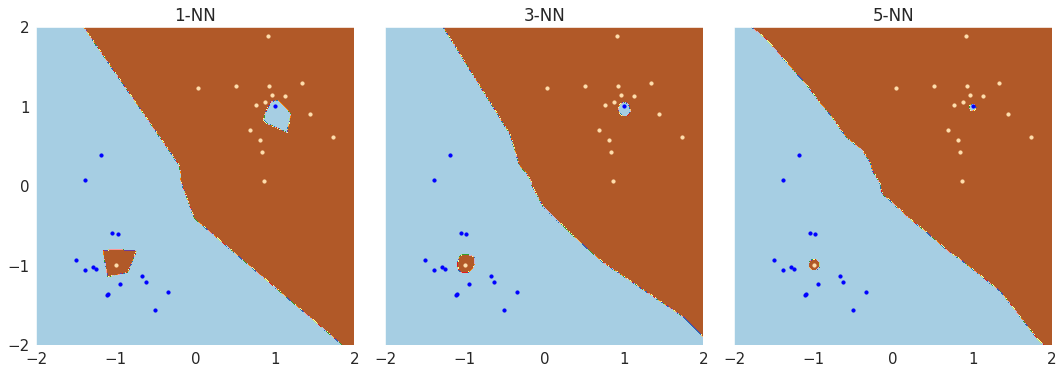
\includegraphics[scale=0.36]{nn-map.png}
    \caption{A visualisation of the decision boundary learnt by the soft $k$-NN
    classifiers, for increasing $k$. The colors in the figure show hard outputs,
    showing the class given the highest probability. Classifiers with high $k$
    are less smooth. Increasing $k$ pushes the decision boundaries towards the
    ``dictionary'' case.}
    \label{fig:knn-map}
\end{figure}

\begin{figure}[!h]
    \centering
    \qquad
    \subfloat[][\centering Natural and Adversarial Accuracies of
    $\mathcal{C}_{k\text{-NN}}$]{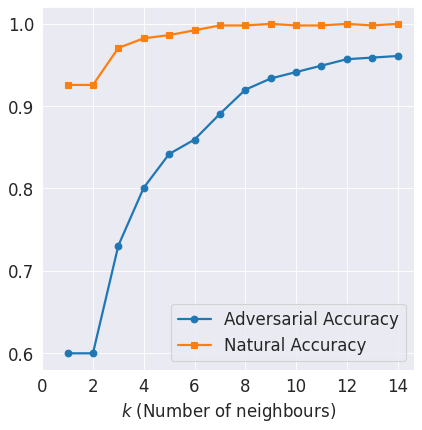
\includegraphics[scale=0.4]{nn-accuracies.png}}
    \qquad
    \subfloat[][\centering Lower bound on Lipschitzness ($\kappa$) of the
    classifiers]{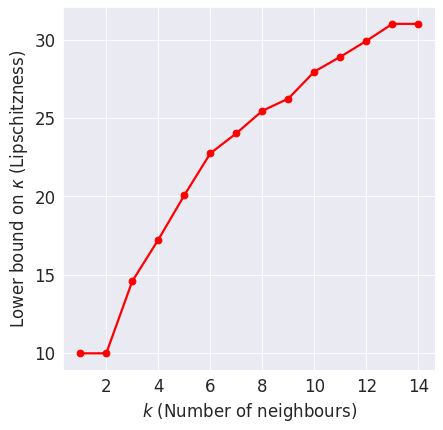
\includegraphics[scale=0.40]{nn-distances.png}}
    \caption{Smoother soft $k$-nearest neighbour classifiers are less adversarially robust.}
    \label{fig:knn-accuracies}
\end{figure}

\section{Lipschitzness bounded by distance to the nearest point, of different label}
\begin{theorem}
    \label{theorem:Lipschitzness-extension-closest-one}
    Let $\mathcal{C}$ be a classifier, and $\mathcal{D}: \mathbb{R}^d \to
    \mathbb{R}_{\geq 0}$ the data distribution, and $c: \mathbb{R}^d \to \Omega$
    be the ground truth labeling function, where $\Omega$ is the set of classes.
    If there exist constants $c_1, c_2, c_{\text{in}}, c_{\text{total}}$ and $R
    \geq r$ and a set $\zeta \subset \mathbb{R}^d$, such that:
    \begin{enumerate}
        \item $c_{\text{ceil}} \geq \mathbb{P}_{\vec{x} \sim \mathcal{D}} \bigg
        [~\underset{\vec{s} \in \zeta}{\bigcup}~\mathcal{B}_R^p(\vec{s}) \bigg ]
        \geq c_{\text{total}}$
        \item $\forall \vec{s} \in \zeta,~~ \mathbb{P}_{\vec{x} \sim
        \mathcal{D}} [\mathcal{B}_r^p(\vec{s})] \geq
        \frac{c_{\text{in}}}{|\zeta|}$
        \item $\forall \vec{s} \in \zeta,~\forall \vec{u}, \vec{v} \in
        \mathcal{B}_R^p(\vec{s}),~c(\vec{u}) = c(\vec{v})$
    \end{enumerate}
    where $\mathcal{B}^p_\rho(\vec{x})$ refers to a $\rho$-radius $l_p$ ball
    around $\vec{x}$. Let S be a training set, obtained by taking $n$ i.i.d.
    samples from $\mathcal{P}$, and labeling each with $c(.)$ with $\eta$
    probability, or some incorrect class with probability $1-\eta$. If a
    classifier $\mathcal{C}$ is such that
    \begin{enumerate}
        \item $\mathcal{C}$ has 100\% training accuracy on $S$. This means it
        gets the correct class on unflipped points, and has also memorized the
        wrong label on flipped points. Further, on each training point, the
        classifier $\mathcal{C}$ is confident on the result at least $\chi$ more
        than the second largest output probability.
        \item $\mathcal{C}$ is locally Lipschitz. We assume that this
        Lipschitzness constant is a decreasing function $\kappa$ of the distance
        to the nearest point of the opposite label. So for each point $\vec{x}
        \in \mathbb{R}^d$ and $\vec{x'}$ in its neighbourhood, with the nearest
        point to $\vec{x}$ with a different label being at a distance greater
        than $L$ in $l_p$ norm,
            \begin{equation*}
                \frac{\llbracket \mathcal{C}(\vec{x}) \neq \mathcal{C}(\vec{x'}) \rrbracket}
                    {\norm{\vec{x} - \vec{x'}}_p} 
                \leq \kappa(L)
            \end{equation*}
    \end{enumerate}
    then,

    \begin{equation*}
        \mathbb{P} \biggl [
        \mathcal{R}_{\text{Adv}}^{R+r-\frac{1}{\kappa(R-r)}}
        (\mathcal{C}) \geq
        c_{\text{total}} 
        \biggr ]
        ~ \geq ~
        (1-c_{\text{ceil}})^{n-|\zeta|}
        \biggl (
            \frac{\eta n c_{\text{in}}}{e}
        \biggr )^{|\zeta|}
        \sqrt{2 \pi |\zeta|}
    \end{equation*}

    The lower bound on the probability might seem highly vacuous at first, but
    it might not be so. With increasing sample complexity, the training set will
    be having a large number of correctly labeled points around an incorrectly
    labeled point, when the Lipschitzness assumption also breaks down if the
    classifier has to memorise the mislabeled point. The above theorem, hence
    should be considered in the light of low sample complexity. If there are
    only a few samples taken from $\mathcal{D}$, then while the highest
    probability density regions will receive points with high probability, there
    will be ``intermediate" probability density regions that can receive a
    mislabeled point, with a correctly labeled point very far off from them.
    This means the network will learn larger regions with the wrong label,
    around such mislabeled points. The above theorem formalises this phenomenon.
\end{theorem}
\begin{proof}
If the sampling (and adding label noise) process results in one mislabeled point
inside each $l_p$ ball of radius $r$ around each point in $\zeta$, and no other
point inside each $l_p$ ball of radius $R$ around each point in $\zeta$, then,
\begin{equation*}
    \mathcal{R}_{\text{Adv}}^{R+r-\frac{1}{\kappa(R-r)}}
    (\mathcal{C}) \geq
    c_{\text{total}}
\end{equation*}
We need to lower bound the probability that this event, denoted as
$\mathcal{E}$, happens. Since we sample $n$ times from $\mathcal{D}$, the
probability that exactly $|\zeta|$ samples result inside each of the $l_p$ balls
of radius $r$, and the rest lie outside the $l_p$ balls of radius $R$, is
\begin{equation*}
        \mathbb{P}(\mathcal{E})
        \geq 
        ~(1-c_{\text{ceil}})^{n-|\zeta|}
        (\eta c_\text{in})^{|\zeta|} \cdot {n \choose |\zeta|} \cdot |\zeta|!
\end{equation*}
Using the inequalities ${n \choose k} \geq (n/k)^k~\text{and}~k! \geq \sqrt{2\pi
k}\cdot(k/e)^k$,
\begin{equation*}
    \begin{split}
        \mathbb{P}(\mathcal{E})
        \geq &
        ~(1-c_{\text{ceil}})^{n-|\zeta|}
        (\eta c_\text{in})^{|\zeta|} \cdot {(n/|\zeta|)^{|\zeta|}} \cdot
        \sqrt{2\pi |\zeta|}\cdot(|\zeta|/e)^{|\zeta|} \\
        = &
        (1-c_{\text{ceil}})^{n-|\zeta|}
        \biggl (
            \frac{\eta n c_{\text{in}}}{e}
        \biggr )^{|\zeta|}
        \sqrt{2 \pi |\zeta|}
        % \biggl (
        %     \frac{\eta n c_{\text{in}}}{e |\zeta|}
        % \biggr )^{|\zeta|}
        % \sqrt{2 \pi |\zeta|}
    \end{split}
\end{equation*}
which is the bound we need.
\end{proof}





\chapter{Early Unsuccessful Experiments}
\label{chapter:failed-exp}

The first subsection of this Chapter covers many of the initial experiments we
did, and failed at. The rest of the subsections detail the other experiments
that shed light on what happens when networks memorize label noise, and
eventually with a few final experiments showing the nature of the worst points
to mislabel.


% \begin{figure}[!h]
%     \centering
%     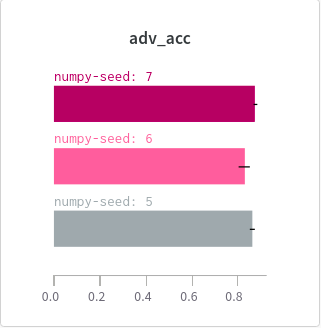
\includegraphics[scale=0.6, trim={10 10 10 10}, clip]{different-poisons-multiple-runs.png}
%     \caption{Only one point from class 5 was flipped to class 6. This was
%     randomly chosen for 3 different runs, and for each run, multiple models were
%     trained, and their accuracy on \emph{targeted} attacks from class 5 to 6 was
%     averaged. The figure indicates that some points are worse for adversarial
%     accuracy compared to others, when mislabeled.}
%     \label{fig:random-runs}
% \end{figure}

\section{Building graphs on training points}

\citet{sanyal2021how} theoretically gives bounds for the adversarial risk by
reasoning that if mislabeled points are placed at high density regions - regions
where if the classifier memorizes the wrong label, will render a large amount of
probability mass in the vicinity of this mislabeled point vulnerable. This was
the inspiration for the algorithm we studied initially: flipping the labels of
training points which come from high probability density areas. The ideas in
this section involve flipping the labels of training points in regions which can
render as much probability mass in their neighbourhood vulnerable as possible.
For datasets like MNIST, there is no reliable way to model the probability
density function given training points, which is why we attempt to resort to
heuristics, based on various combinations of representations of points with
different ways of selecting points. This will be explained in detail in the
following paragraphs. The algorithms discussed in this section require a few
definitions.

\begin{definition}
    Given a set of points, $S=\{\vec{x_i}\}_{i=1}^m$, the Class-Graph of this
    set of points $G_\gamma^{p}(S)$ is defined as the undirected graph
    $G_\gamma^{p}(S) = (\{1..m\}, E_\gamma^p(S))$ where
    \begin{equation*}
        E_\gamma^p(S) =
        \{\{i, j\}~\mid 0 < i < j \leq m~\wedge~
        \norm{\vec{x_i}-\vec{x_j}}_p \leq \gamma \}
    \end{equation*}
    \label{def:class-graph}
\end{definition}
Intuitively, a class-graph of a set of points is an undirected graph connecting
every two points closer than a threshold $\gamma$, under some norm $p$.

The algorithm is based on the following idea: For each class of the dataset, we
build class-graphs in some representation space. The degrees of various points
are now considered to be a heuristic for the probability density at each point.
We then use one of the two selection strategies outlined below to select
vertices from class graphs, which will then be label-flipped. When we refer to
label-flipping, we simply will change each label selected to be of the next
class, cyclically. The adversarial accuracy of the resultant model will then be
evaluated in a targeted manner, by carrying out targeted PGD attacks from each
class to the next one.

\subsection*{Selection Algorithms}
The following two algorithms are the selection algorithms we experimented with.
Each of them take in an undirected graph, and select a given number of vertices
from it. Let $\Delta$ be the maximum degree in the given graph.
\begin{enumerate}
    \item Algorithm \ref{alg:greedy-selection}: We simply select $b$ nodes with
    the highest degrees
    \item Algorithm \ref{alg:log-delta}: A $(\Delta + 2)$-approximation to the
    dominating set problem ($\Delta$ is the largest degree in the input graph),
    for a budget number of vertices in the dominating set.
    \citep{dominating-set} proves the approximation factor for the full
    dominating set problem, and the proof for this budget-version follows form
    it.
\end{enumerate}

\begin{algorithm}[!h]
\caption{Greedily Selecting vertices}
\begin{algorithmic}[1]
\Procedure{Greedy-Selection}{$G, b$}
    \State Degrees $\gets [\text{degree(i) for i in}~V(G)]$
    \State Selected-Vertices $\gets$ Sort-By-Val($\{1..|V(G)|\}$, Val=Degrees)[-b:]
    \State \Return Selected-Vertices
\EndProcedure
\end{algorithmic}
\label{alg:greedy-selection}
\end{algorithm}

\begin{algorithm}[!h]
\caption{$(\log \Delta + 2)$-approximation to the dominating set problem}
\begin{algorithmic}[1]
\Procedure{Smart-Greedy-Selection}{$G, b$}
    \State $n \gets |V(G)|$
    \State $S \gets \phi, D \gets \phi, U \gets \{1..n\}$   \Comment{$\phi$ refers to the empty set}
    \While{$b > 0~\wedge~U \neq \phi$}
        \State choose $v \in \underset{x \in D\cup U}{\arg\max}|{U\cap (\{x\}\cup N_G(x))}|$
        \Comment $N_G(x)$ is the set of points in $G$ neighbouring to $x$
        \State $S \gets S \cup \{v\}$
        \State $U \gets U \setminus (\{v\}\cup N(v))$
        \State $D \gets D\cup({U\cap (\{v\}\cup N_G(v))})$
        \State $b \gets b - 1$
    \EndWhile
    \State \Return S
\EndProcedure

\end{algorithmic}
\label{alg:log-delta}
\end{algorithm}

It is a valid question as to why we ran 2 different algorithms: one where only
high degree nodes are selected (greedy strategy), and one which is an
approximate solution to the modified dominating set problem discussed before.
When we select only select high degree points, we might be rendering points from
the same neighbourhood vulnerable, which the second algorithm avoids.

\subsection{Building graphs on input space}
The first attempt was to build \emph{Class Graphs} on each class of the MNIST
dataset, and for each class, pick vertices from the graph to flip labels. For
now, we do not concern ourselves with the label we flip to. Each label that has
to be flipped is simply set to the next value cyclically.

The procedure we followed was as follows:
\begin{enumerate}
    \item Produce \emph{Class Graphs } for all classes on the MNIST dataset
    \item Select $b$ points to flip using one of the 2 selection algorithms
    \item Change the labels of the selected points
    \item Train networks on the \emph{poisoned} datasets
    \item  Randomly select $b$ points to flip, and train and evaluate the
    networks on them to have a random baseline to compare with
\end{enumerate}

As previously mentioned, the idea behind the above algorithms on the \emph{Class
Graphs} is that we want to select points that can render as much amount of
probability mass \emph{adversarially vulnerable} as possible. Since we do not
have a reliable method of density estimation, we select points that have a large
number of neighbouring points, as a heuristic.


Surprisingly, the results showed that not only did the above strategies yield
networks that had adversarial errors comparable to the random strategy (i.e.,
they are no better), rather, they were strictly \emph{inferior}. Networks
trained on poisoned datasets modified using the above strategies are more robust
than the ones trained on the same dataset but with random label noise. The next
few subsections illustrate attempts to do the same in different subspaces which
are more feature rich, since it might very well be the case that looking at the
proximity of points in the input representation is sub-optimal for this. One
strong reason why this might be the case is the inter-point distances of the
points in practical datasets we experimented with: MNIST. The distances between
points is far, far more than the perturbation budget $\rho$. Figure
\ref{fig:inter-point-distances} illustrates this.

\begin{figure}
    \caption{Figure showing the distribution of the inter-point distances in
    class 0 of the MNIST dataset}
    \label{fig:inter-point-distances}
\end{figure}

\subsection{Using Low Rank representations}
Principal Component Analysis (PCA) is a popular dimensionality reduction method.
It aims to find $d_\text{low-rank}$ orthogonal directions, given $d$ dimensional
data points, such that the dataset has the highest variance along these
$d_\text{low-rank}$ directions. The dimensionality reduction is then done by
first centering the data to have $0$ mean, and then projecting the data points
onto each of the $d_\text{low-rank}$ vectors, getting $d_\text{low-rank}$
dimensional representations for each of the points. These $d_\text{low-rank}$
directions are obtained by finding out the eigenvectors corresponding to the
$d_\text{low-rank}$ highest eigenvalues of the covariance matrix of the data
distribution. In practice, the mean and the covariance matrix are
\emph{estimated} from the given data points. These low-dimensional
representations yielded by PCA are generally referred to as \emph{low-rank}
representations as well.

We calculated the low-rank representations of points in the MNIST training set,
and built Class-Graphs on these low-rank representations. This experiment did
not yield any conclusions. In certain cases, it performed better and in certain
cases worse, than the random baseline, which is not conclusive of anything.

\subsection{Using the feature representations of a trained network}
The next attempt was to consider the representations learnt by a trained network
on the dataset. Networks are able to extract rich features, that heavily
correlate with the label. It might be the case that selecting points that are
closer in \emph{feature space} might perform well. This attempt too, did not
yield anything.

This was rather a bit short sighted, since we later realised, and experimentally
verified as well, that networks memorize the false labels by learning very
different feature representations, compared to other points in the vicinity,
which have a different (correct) label.


\subsection{Using the feature representations of a trained network as well as input space}

The final experiment in this direction was to select points that are high-degree
both in the input as well as feature space. We select $2b$ number of points from
input as well as feature space. The greedy algorithm was employed for this,
since the other one almost selected the same set of points, for the small
budgets we had. We then select $b$ points from the intersection of the set of
points selected by both the algorithms.

The above also did not yield definitive results.


\section{Min Coloring trick}
If we could fit one model with each training set point flipped, then we could
iterate over all such models and check which mislabelled points cause the
largest drop in adversarial accuracy. In this experiment, we build graphs over
the training set points of MNIST which belong to class 5, having one edge
between points closer than $\gamma$ in $l_\infty$ distance. We then solve an
extension of the minimum coloring problem on this graph, where even two adjacent
nodes cannot be assigned the same color, and so cant second neighbours. We only
need an approximate solution, which ensures that neighbours or second neighbours
are not assigned the same color. The idea is to fit a network $\mathcal{N}$
mapping these points to the colors. After $\mathcal{N}$ memorizes the colors, we
iterate over every point in class 5, attempting to assign a score to each point.
The score for a point $x$ is determined by the number of its neighbours which
were rendered vulnerable to $x$, which is estimated by the number of $x$'s
neighbours such that we can carry out a \emph{targeted} attack from them, and
flip the network's output to the color assigned to $x$.

The idea behind the above experiment is that the network might be memorizing
similar regions of the wrong label for mislabelled points in the poisoned
dataset setup as different coloured regions when we assign colors to the
training points. Further, the reason why we ensure that neighbours and second
neighbours are not assigned the same color is that when we start out with a
training point $x$, with an assigned color $c(x)$, we need to carry out a
targeted attack from this point to the color of one of its neighbours, hence if
2 neighbours share the same color, we cannot be sure which region (pertaining to
which of these neighbours) the attack settled at.

Next, we flip the labels of the training points in class 5 with the largest
scores assigned by the above algorithm. The resulting network's adversarial
accuracy is estimated on class 5 only, and that too in a targeted fashion, attempting attacks that flip the network's output from 5 to 6, precisely.

\begin{figure}
    \centering
    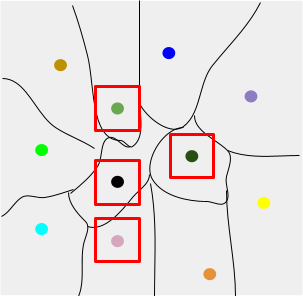
\includegraphics[scale=0.4, trim={0 0 0 0}, clip]{thesis-coloring-trick.png}
    \caption{Idea behind using different color labels for each point in a specific class, and getting a network to memorize the assigned labels. The black lines show the decision boundaries learnt for the different colors, and red boxes show the points which are vulnerable because of a boundary passing through the $l_\infty$ balls around those points.}
\end{figure}

\emph{The above experiment was compared to the random strategy, where randomly chosen points from class 5 (same fraction of points mislabeled, for comparison). The random strategy still performed better, compared to points selected by the above algorithm. This hints towards the idea that there are points, and a large number of them, such that the network not only learns a wrong region around them, but probably learns stretched out, far reaching regions from the decision boundary that it would have learnt on a clean dataset.}



\chapter{Experimental results}
\label{chapter:experiments}

\section{Toy Distribution}

The initial (failed) experiments we tried were based on the fact that placing
mislabeled points with the idea of having high probability mass in the vicinity
might be optimal. These experiments are discussed in Chapter
\ref{chapter:failed-exp}. To develop a better understanding of how neural
networks fit mislabeled points, what exactly is the cause of the huge drop in
their vulnerability when \emph{random} label noise is introduced into the
dataset, and also why the highest probability density regions are not the best
to label-flip, we carry out some controlled experiments in this chapter. Some of
the following experiments utilize a toy dataset which consists of two classes,
with the instance space being $\mathbb{R}^d$. $n$ samples are generated from the
gaussian mixture

\begin{equation*}
    \mathcal{P}_\text{toy}(\vec{x})=\frac{1}{2} \mathcal{N}(\vec{x}|-\mu \vec{1}_d,
    \sigma^2 I_d) + \frac{1}{2} \mathcal{N}(\vec{x}| \mu \vec{1}_d, \sigma^2 I_d)
\end{equation*}
and labelled with the ground truth labeling function 
\begin{equation*}
    c_\text{toy}(\vec{x}) = \llbracket
    \vec{x}^T.\vec{1_d} \geq 0 \rrbracket 
\end{equation*}
to create a dataset, where $\mathcal{N}(\cdot \mid \vec{m}, \Sigma)$ refers to
the normal distribution with mean $\vec{m}$ and covariance matrix $\Sigma$. This
dataset is denoted as $\mathcal{D}_\text{toy}$. From this, we create a
\emph{poisoned} dataset $\mathcal{D}_\text{toy}^r$ where we place $b$ mislabeled
points for each class, at $r$ distance from the means of the 2 classes,
(uniformly sampled at $r$ distance). We drop many of these details from the
notation of $\mathcal{D}_\text{toy}$ for clarity. We are \emph{placing}
mislabeled points, and not \emph{flipping} since that provides greater control
over toy experiments.

\begin{figure}[!h]
    \centering
    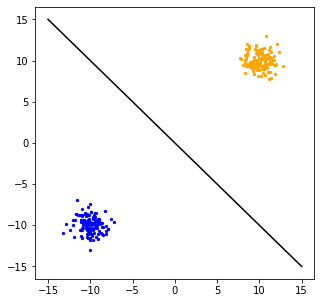
\includegraphics[scale=0.4]{sample_data}
    \caption{Toy data distribution with $d=2,~\mu=10,~\sigma^2=1,~d=2$}
    \label{fig:data_sample}
\end{figure}

Figure \ref{fig:data_sample} shows samples from $\mathcal{D}_\text{toy}$ with
$\mu=10, \sigma^2=1, d=2$.


\subsection{Toy distribution with points far away from the decision boundary}

Here, we aim to study the vulnerability of networks when $\mu \gg \sigma$. The
decision boundary given by $\vec{x}^T.\vec{1_d} = 0$ is far away from where the
points are located. For now, this notion of being far away is not well defined.
But what we want to study is the effect on the adversarial vulnerability of
networks when poisons are very far away from the boundary that these networks
would have learnt otherwise in the absence of poisons. This decision boundary
that the classifier would have learnt in the absence of poisons will be refered
to as the \emph{natural boundary}. We attempt to keep the boundary far away so
that the networks do not stretch the natural boundary, in order to accommodate
poisons. The networks should be learning clean, new pockets around the
mislabeled points, where they give the wrong answer. It is a valid question as
to how we might know whether the affect we want to avoid is actually not
happening, and that networks are learning closed pockets around mislabeled
points. For this, we found an experimental trick: mislabeling points to a third,
new class that is not present in the dataset. Since this class is not present in
the training set, when the network memorises them, it cannot stretch the natural
decision boundary to do so. The training setup for this case, with the new class
introduced, is the exact same, with one extra logit added to the output layer of
the network.

The adversarial accuracy of models trained in this experiment were evaluated
using an $l_\infty$ PGD adversary, with an attack radius of 0.2.

\begin{figure}[!h]
    \centering
    % 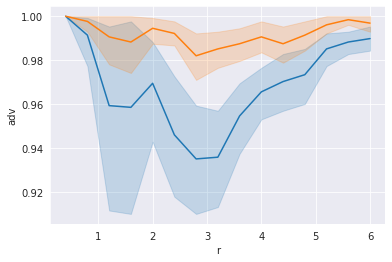
\includegraphics[scale=0.75]{normal_training_toy_dataset}
    \subfloat[][\centering Poisons have labels set to the opposite
    class]{{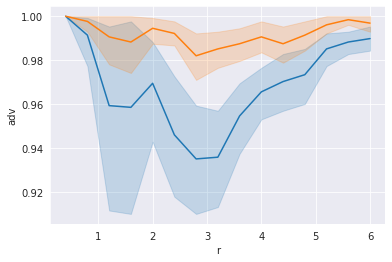
\includegraphics[scale=0.45]{normal_training_toy_dataset}}}
    \qquad
    \subfloat[][\centering Poisons have labels set to a third, new
    class]{{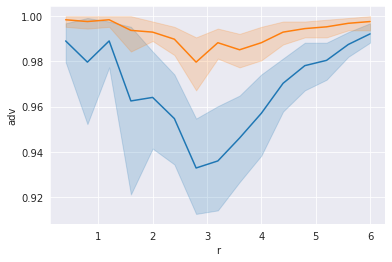
\includegraphics[scale=0.45]{normal_training_toy_dataset_with_3rd_class}}}
    \caption{\fcolorbox{orange}{orange}{\rule{0pt}{3pt}\rule{3pt}{0pt}} is the
    test accuracy \fcolorbox{blue}{blue}{\rule{0pt}{3pt}\rule{3pt}{0pt}} is the
    adversarial accuracy. $r$ axis represents the distance from the means of the
    gaussians where mislabelled points (poisons) were placed. Setting wrong
    labels to a third class produces a curve very similar to the case where
    labels were set to the opposite class for poisons. Multiple models were
    trained, and randomisation was also done on the poisons placed for each run,
    which is what the confidence intervals and mean curves are representative
    of.}
    \label{fig:far-gaussian-curve}
\end{figure}

Figure \ref{fig:far-gaussian-curve} shows the results of two runs ($d=16, b=2,
\sigma^2=1, \mu=10$) with 64 points in the training set (including the
mislabeled points). We fit networks to different toy datasets with the $r$
parameter being varied. Reiterating, $r$ is the distance from the means from
which the mislabeled points are placed (in this case, 2 mislabeled points per
class). The results are summarised as follows:

% \todo{what is the experiment ??}
\begin{enumerate}
    \item Two data points with label $0$ were placed near $\mu\vec{1}_d$ and two
    points labelled with $1$ were placed near $-\mu\vec{1}_d$. Classifiers were
    then trained to overfit to this dataset (achieve 100\% training accuracy).
    The curve shows that adversarial accuracy first decreases and then
    increases, as poisons are placed farther and farther away from the means of
    the Gaussians. This is even more evidence for the conjecture that placing
    mislabeled points in the highest probability density regions does not hurt
    the adversarial accuracy by the largest factor.
    \item The above experiment was repeated, but the label-flipping is done to a
    third, new class. This was to see whether the drop in adversarial accuracy
    primarily stems from learning more complex decision boundaries in the first
    experiment where the poisons were labeled with the opposite class, or the
    vulnerability is equally bad when the classifier has to learn new regions
    with the third class as the label. The curve obtained in this case is very
    similar to the previous experiment, indicating that regions memorized to be
    of the opposite class is not worse for the adversarial accuracy, in
    comparison to the case where the network is forced to memorize new regions
    % \todo{Describe the results here and their significance}
\end{enumerate}

For the exact same setup, when the dimensionality $d$ is increased, the
adversarial accuracy quickly shoots up to one and the curve becomes flatter (as
shown in the next section). Since standard datasets are generally high
dimensional, the next section involves 64 dimensional toy data.

  
   
% \subsection{Theorem capturing the tradeoff - Lipschitzness bounded by
% inter-point distances}

% Given a dataset $\mathcal{D}$, drawn from a distribution $\mathcal{P}$ and
% labeled using the ground truth labeling function $c$, we, as attackers are
% allowed to flip one label in this entire dataset. In this section, we attempt to
% lower bound the adversarial risk when the attacker has a budget of 1 point, with
% the following assumptions:
% \begin{enumerate}
%     \item Given a point $\vec{x_1}$ which the network $\mathcal{C}$ has fit with
%     confidence $\chi$ more than the second most confident class, and another
%     point $\vec{x_2}$ which is closest to $\vec{x_1}$ of another class in the
%     training set $\mathcal{D}$, under some norm $p$. We assume the Lipschitzness
%     of a network is constrained by a decreasing function $\phi$ of the distance
%     to the nearest point of another class:
%     \begin{equation*}
%         \frac{\norm{\mathcal{C}(\vec{x}) - \mathcal{C}(\vec{x_1})}_p}
%         {\norm{\vec{x} - \vec{x_1}}_p} \leq \phi (\norm{\vec{x_1} - \vec{x_2}}_p)
%     \end{equation*}
%     \item There exists a finite set $\zeta \subset \mathbb{R}^d$, s.t. $\forall
%     \vec{x} \in \zeta$,
%     \begin{equation*}
%         \mathbb{P}_{\vec{x'}\sim\mathcal{P}}[\vec{x'} \in
%         \mathcal{B}_r^p(\vec{x})] \geq c_1,~
%         \mathbb{P}_{\vec{x'}\sim\mathcal{P}}[\vec{x'} \in
%         \mathcal{B}_{R(\vec{x})}^p(\vec{x})] \leq c_2
%     \end{equation*}
%     and
%     \begin{equation*}
%         \mathbb{P}_{\vec{x'} \in \mathcal{P}}\biggl[\vec{x'} \in
%         \mathcal{B}_{r+\rho+\tau(R(\vec{x})-r)}^p(\vec{x})\biggr] \geq c
%     \end{equation*}
%     \item The attacker is given $\zeta$. While we cannot reliably sample a point
%     which lies inside a particular region, we can query whether a point
%     $\vec{x}$ lies inside or outside any $l_p$ ball around a member of $\zeta$
% \end{enumerate}
% then, the adversarial risk when the label-flipper is allowed to modify any label
% can be lower bounded as follows:
% \begin{equation}
%     \mathcal{R} \geq c~\text{with probability at least}~
%     \sqrt{2\pi|\zeta|}\cdot\biggl(\frac{c_1 n}{e}\biggr)^{|\zeta|}\cdot(1-c_2|\zeta|)^{n-|\zeta|}
%     \label{thm:crafting-noise}
% \end{equation}
% \begin{proof}
%     Given the assumptions, we need to simply lower bound the probability that at
%     least 
% \end{proof}

\subsection{Toy distribution with points close to the decision boundary}

Here, we further carry out experiments on the toy dataset, this time with higher
dimensionality (64 dimensions), and vary $\mu$ and $r$, to observe how the
adversarial accuracy of a fit network changes. This time, we are interested in
observing the affects when mislabeled points are placed close to the decision
boundary as well. The increase in dimensionality is because we need to ensure
that the effects we see are not merely artefacts of low dimensionality (the
results of the previous section are such artefacts, since for the same strength
of the adversary, the accuracy turns out to be 100\% for $d=64$).

Differences in the adversarial accuracies, between the cases where we flip to
the other class, and when we flip to a 3rd class, are \emph{larger} when the
means are \emph{closer}.

We vary $\mu$ and $r$, fit networks for each case, and estimate the adversarial
accuracy of the fit network. We carry out these experiments for $d=64$, with a 4
layer fully connected, ReLU activated network. After creating the poisoned
dataset, we fit networks with the stated architecture to these poisoned
datasets, and evaluate their adversarial as well as natural accuracies. The
results clearly indicate that placing mislabeled poisons near the mean is the
\emph{worst} for having high adversarial error. There is high variance in the
adversarial accuracy of models given vanilla training, hence we ran multiple
seeds for each setup.

For the case where the means were very far apart, the adversarial accuracy was
the highest, and the poisons had almost no effect. Closer the class-means get,
lower the adversarial accuracy.

We also made another change to the setup, like in the previous section, and
repeated the above experiments. The training setup is the exact same, except
that this time, we mislabel points to a \emph{third} class, which is not present
in the dataset. The network is given one extra unit in its output layer, and all
hypterparameters are preserved. All of the relative trends we observed above
were observed again, but this time the networks had \emph{higher} adversarial
accuracies for cases where mislabeling was done to a third class.

Another point to note is that while the natural accuracies of the networks also
showed the same trends as the adversarial accuracies, these are on a very
different scale, with all values being upwards the 99\% accuracy mark.

\begin{figure}[!h]
    \centering
    % 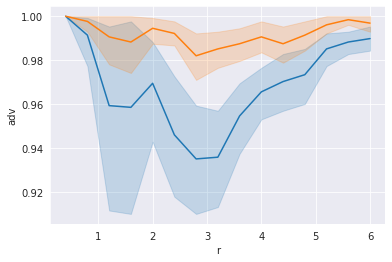
\includegraphics[scale=0.75]{normal_training_toy_dataset}
    \subfloat[][Adversarial Accuracies]{{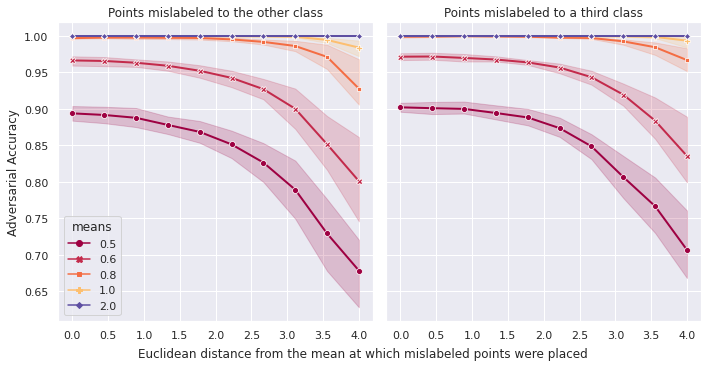
\includegraphics[scale=0.5]{toy.png}}}
    \qquad
    \subfloat[][Natural
    Accuracies]{{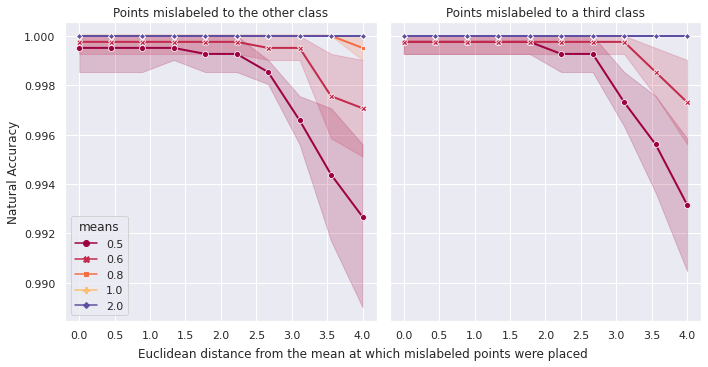
\includegraphics[scale=0.5]{toy-but-natural-accuracies.png}}}
    \caption{$d=64, b=2, \sigma^2=1.0$; $2$ mislabeled points were placed per
    class. As before, randomisation is over training multiple models with
    different initialisations, and placing poisons randomly sampled at a given
    $r$ from the means.}
    \label{fig:poison-toy-experiments}
\end{figure}

We can derive the following conclusions from the above experiments:
\begin{enumerate}
    \item Adversarial accuracy is hurt more by mislabeling to a class whose
    decision boundary lies close. This is indicated by the fact that when we
    flipped the label to a new, 3rd class, the adversarial accuracy was better
    than when we flipped the label to the other class.
    \item Placing the mislabeled points at the highest probability density
    regions is ineffective when our intention is to increase the adversarial
    error. In fact, in many of the above experiments, the networks simply did
    not fit the mislabeled points placed at these high density regions. This is
    further motivation to not place mislabeled points in such regions, since we
    cannot expect the victims' models to memorize these points. They can simply
    use \emph{early stopping}, and their models will be as good in adversarial
    accuracy as models that would have been trained on clean datasets.
    \item When the class-means are closer to each other, the adversarial error
    is \emph{higher}. This indicates that the most adversarially vulnerable
    networks simply do not memorize a closed region around mislabeled points,
    rather they tweak the decision boundary to include the mislabeled points,
    rendering large amounts of probability mass vulnerable ``on the way". Figure
    \ref{fig:pockets-or-tweaks} shows a visualisation of this. Further
    experiments add strong evidence in support of this claim.
\end{enumerate}

Till this point in this chapter, we do not have enough insights to exactly
understand what might be an optimal strategy to flip labels.

% \todo{Create a visualisation of the distribution}


% \subsection{Fitting low dimensional poisoned datasets}

% \emph{This section does not align directly with the problem at hand, and can be skipped}

% SGD did not manage to learn networks that get a 100\% training accuracy on the
% poisoned dataset for the case of 2 dimensional Gaussians when the poisons are
% very close to the means. Instead, the classifier resorts to a simple, almost
% linear decision boundary. The following was an experiment to hash the datapoints
% using the function in Listing \ref{lst:hash} and get SGD to learn complex
% decision boundaries when the sense of proximity of correctly labelled points is
% destroyed. Points in the instance space which are close to each other in each of
% the clusters are no longer close after mapping them to a different space, and
% the classifier is forced to resort to complex decision boundaries if a low loss
% is to be achieved. Figure \ref{fig:hash-trick} shows the decision boundaries
% learned. SGD managed to hit a 100\% training accuracy, and the same training
% setup without the hash function was not able to do the same.
% % \todo{what does this mean ?}
% \citep{rahaman2019spectral} show that SGD learns classifiers that are biased
% towards first capturing lower frequency components, and then learning higher
% frequency ones, even if the amplitudes of these low frequency components is
% smaller. Further, they experiment with a dataset generated using a low frequency
% function in 1 dimension, and embed it in 2D on increasingly complex manifolds.
% High frequency components were learned faster when this manifold has larger
% complexity, and this might be happening here as well. Passing the data points
% through the hash embeds this data in a higher dimensional space, in a complex
% manifold, where high frequency components are easier to capture.
% % {\color{red} Further, they also show that these high frequency
% % components are learned faster or slower depending on how complex the
% % representation of the data is (more complex representations lead to the network
% % learning higher frequency components faster), which is likely what is happening
% % here.}
% % \todo{not sure what the red line means }
% \begin{figure}[!htb]
%     \centering
%     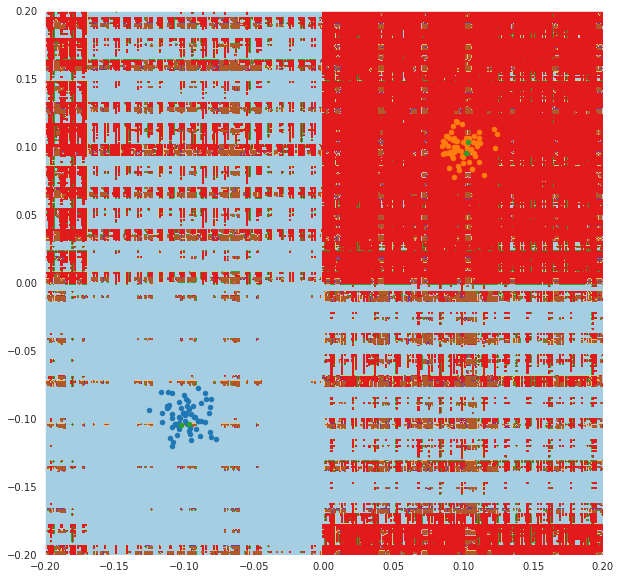
\includegraphics[scale=0.6]{hash_trick}
%     \caption{Map showing a classifier's decision boundaries and data points when the classifier is shown points after passing through the aforementioned function. The two classes are in red and blue, and green is the third class that poisons were labelled with.}
%     \label{fig:hash-trick}
% \end{figure}

% \lstset{language=Python}
% \lstset{frame=lines}
% \lstset{caption={\centering Function used to map data points $\in \mathbb{R}^d$ to bit sequences that are shown to the network}}
% \lstset{label={lst:hash}}
% \lstset{basicstyle=\footnotesize}
% \begin{lstlisting}
% def hash(x): # x is a floating point number
%     P = 941
%     LN = 2^BITS
%     x = round_down(x * LN) % P
%     return binary_representation(x, length=BITS) 
% \end{lstlisting}

% \subsection{Toy experiment with Lipschitzness constraints on the network}
% This experiment is on the toy dataset, with $d=16$. We constrain the
% Lipschitzness of the network trained on the poisoned dataset, using spectral
% normalization on every layer. The last layer's spectral norm is varied, and the
% results show that the higher this spectral norm, lower the adversarial accuracy
% of the network trained on the poisoned datasets. Hence, spectral normalization
% as a regularization leads to higher adversarial accuracy. Poisons which were
% placed very close to the mean of the gaussians, were not even memorized by
% networks having a lower spectral norm, which acts as a natural defence against
% mislabelled points. Figure \ref{fig:Lipschitzness-toy} shows the results of the
% above experiment.

% \begin{figure}[!h]
%     \centering
%     \includegraphics[scale=0.43, trim={0 50 0 0}, clip]{Lipschitzness_toy}
%     \caption{Accuracies of the networks trained with different spectral normalization constraints. Distance of the mislabelled points from the mean is written inside the sub-figures. For points closer than 2.8, the networks dont memorize the training set entirely, hence that part has not been shown.}
%     \label{fig:Lipschitzness-toy}
% \end{figure}


\section{The worst poisons are not the ones producing pockets with the wrong label}

% The following experiments indicate that rather than having poisons having 

\subsection{Flipping to an 11th class in MNIST}

Similar to the approach we took for toy experiments, here we attempt to study
classifiers which memorise the poisoned MNIST dataset. We first randomly select
10 points per class from the MNIST dataset which will be label-flipped, and then
we fit 2 different classifiers: one classifier is fit with the mislabled points
set to the next class in the dataset, and the other classifier, with one extra
logit added in its output layer, is fit with the mislabeled points set to an
11th class, which is not present in the dataset. Adversarial accuracy evaluation
is untargeted for these experiments.

\begin{table}[h!]
\centering
\begin{tabular}{|c | c|} 
 \hline
 Poisoning Experiment & Adversarial Accuracy(\%) \\ [0.5ex] 
 \hline\hline
 Mislabeling to next class & $36.46 \pm 4.42$ \\
 \hline
 Mislabeling to an 11th class & $41.51 \pm 4.26$\\
 \hline
\end{tabular}
\caption{Adversarial Accuracies of networks when poisoning is done to a new
class compared to the case when poisoning is done to the next class cyclically.
The accuracy was evaluated against an $l_\infty$ PGD adversary with an attack
radius of $0.1$. Randomisation in the above results is over model
initialisation. For each run, the same points in MNIST are label-flipped.}
\label{table:mnist-class-10}
\end{table}

Table \ref{table:mnist-class-10} shows the results of this experiment. \emph{The
network trained with points flipped to the 11th class had a much higher
adversarial accuracy compared to the other network.} This indicates that the
poor adversarial accuracy of models trained with random label noise is probably
because of the mislabeled points stretching the decision boundary, and rendering
large amounts of probability mass vulnerable on the way. We ran the above
experiment with other randomly selected points to label-flip as well, and the
results show the same trend.


% \begin{figure}[!h]
%     \centering
%     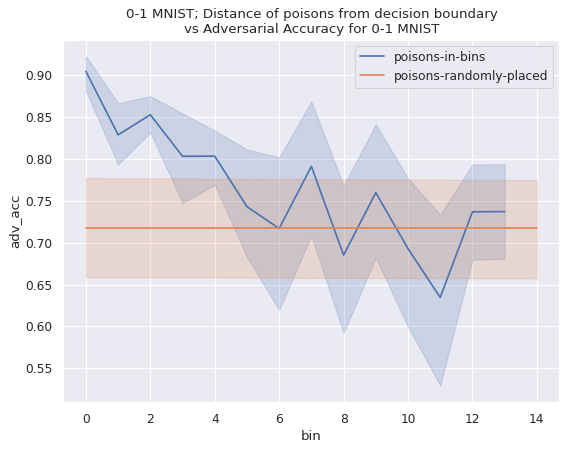
\includegraphics[scale=0.6]{pgd-path-scoring}
%     \caption{0-1 MNIST: The orange curve (baseline) shows the adversarial accuracy of the network when mislabeled poisons are randomly selected. The blue curve shows the adversarial accuracy of different networks trained on poisoned datasets, where the mislabeled poisons were placed at increasing distances from the decision boundary ($x$ axis). The $x$ axis (labeled "bin") is only an ordinal value, and higher values on this axis represent poisoned datasets where the mislabeled points are at greater distances from the decision boundary that the network would have otherwise learnt on a clean dataset.}
%     \label{fig:pgd-path-scoring}
% \end{figure}


% \subsection{Detecting Adversarial examples/mislabeled points}
% This section concerns with 2 experiments:
% \begin{enumerate}
%     \item We fit a network to the poisoned data, and find out the feature
%     representations produced by the network for both the poisoned as well as
%     clean datapoints. We then iterate over the test set points, and find out
%     adversarial examples for each test point. These adversarial examples', as
%     well as the original test points' feature representations are calculated,
%     and their \emph{difference} is projected onto the top 60 PCA components of
%     the a. poisoned datapoints and b. clean datapoints. We find that this
%     difference in representations has larger components along the 
% \end{enumerate}
% The network might be memorizing mislabelled points by having very distinct
% feature representations for them, compared to the clean ones. In this
% experiment, we attempt to 

\section{Analysis using adversarial paths}


\begin{figure}[!h]
    \centering
    % 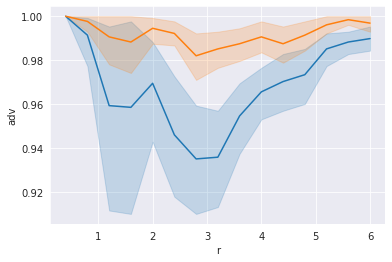
\includegraphics[scale=0.75]{normal_training_toy_dataset}
    \subfloat[][\centering Network learning a ``pocket" around a mislabeled
    point]{{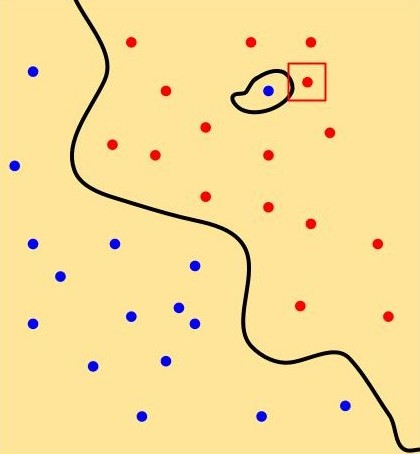
\includegraphics[scale=0.30]{thesis-learning-pockets-or-tweaking-boundary-1}}}
    \qquad
    \subfloat[][\centering Network teaking the decision boundary to
    ``accommodate" a mislabaled
    point]{{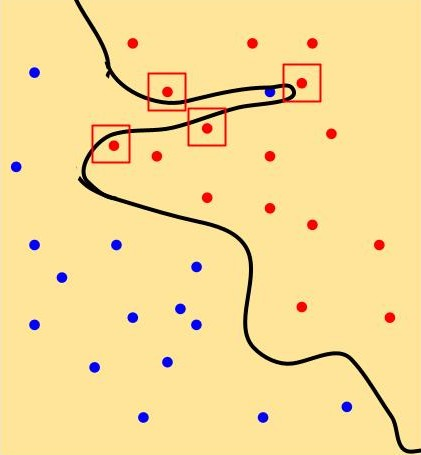
\includegraphics[scale=0.30]{thesis-learning-pockets-or-tweaking-boundary-2.jpg}}}
    \caption{The above figure shows two different ways in which a classifier
    could memorize a mislabeled point. If the decision boundary is tweaked to
    accommodate a mislabeled point, it could lead to much higher adversarial
    errors, compared to the other case.}
    \label{fig:pockets-or-tweaks}

\end{figure}




The following section descibes a series of experiments, which reveal why the
random strategy performs surprisingly well in searching for poisons, and also
sheds light on the nature of training points which when mislabeled, cause a
massive drop in the adversarial accuracy of the model.

The first experiment shows the result for a binary classification problem, with
the MNIST dataset's classes 0 and 1 only. The other case shows the same
experiment done on the full MNIST dataset. The experiments also reveal why we
will always get good enough results (i.e., high adversarial error) while
randomly selecting points to label-flip, because it turns out that points
responsible for huge drop in adversarial accuracy when mislabeled are very large
in number.

\subsection{Finding a path from a point to the boundary}

A requirement to the experiments that follow is a procedure to find a path from
a data point to the decision boundary of a given classifier. For instance, if we
are given a classifier trained on the full MNIST dataset, and are given a
data-point $\vec{x}$ (i.e., some handwritten digit), then we need to find a path
(the shortest path ideally) from this datapoint to the decision boundary. We
might also have a constraint: finding a path to the decision boundary of the
current data point's class, and a target class. Further, this path is
unconstrained, and we are not concerning ourselves with finding such a path that
completely lies inside a certain region, such as an $l_p$ ball of specific
radius around the input $\vec{x}$. We will carry out an \emph{unbounded}
gradient descent attack, and record all the adversarial examples we get on the
way.

For a small step size $\omega$, we make gradient ascent updates on the input
image that is plugged into a model, by backpropagating gradients from the loss,
all over to the inputs. During these gradient updates, unlike Projected Gradient
Descent, we do not project the updated input back into an $l_p$ ball of radius
$\rho$ around the original input. After every update, we record the updated
input. This procedure terminates when the output of the classifier is flipped,
or when some maximum number of steps have already been taken. We will call this
procedure \emph{untargeted-unbounded-gradient-descent}.

When we have several classes, it makes sense to study the effect of poisons by
evaluating the adversarial accuracy of the model using targeted attacks from the
original class of the poisons, to the class the poisons were mislabeled to. For
instance, if some points in class 9 of the MNIST dataset were mislabeled to
class 0, then it makes sense to evaluate the the impact of these poisons by
estimating the robustness of the resultant model using targeted adversarial
attacks from class 9 to class 0. We hence, find out paths in multi-class
settings by recording the path from a given data point to a target decision
boundary. We will call this procedure \emph{targeted-unbounded-gradient-ascent}
\ref{algorithm:unbounded-gd}.

We will refer to the paths traced out by the above algorithms as
\emph{adversarial paths}.

Interestingly, when we found out the adversarial paths for some of the below
experiments, we came across label noise already present in MNIST. This is
illustrated in figure \ref{fig:pgd-path-examples}. We selected points closest to
and farthest from the decision boundary, and plotted them out. Many of the
points closest to the decision boundary already have label noise. Adversarial
paths were found out from each class to the next, in a targeted manner, for this
analysis.

\begin{figure}
    \centering
    \subfloat[][5 points per class closest to the boundary of the next
    class]{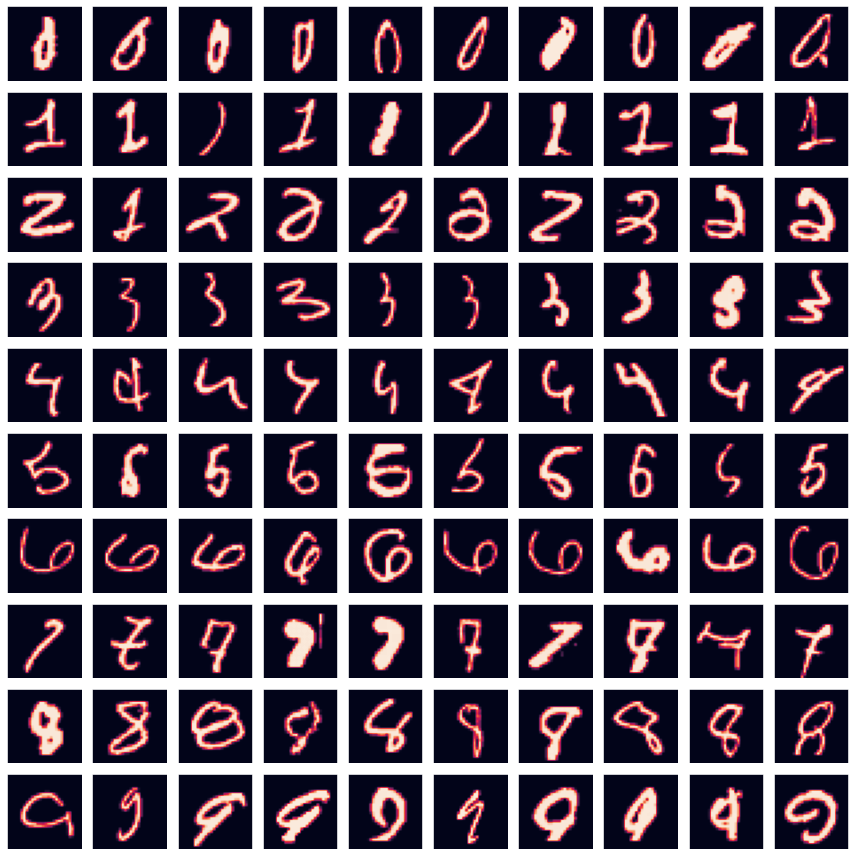
\includegraphics[scale=0.37, trim={425 0 0 0}, clip]
    {mnist-close-to-boundary.png}\label{subfig:close}}
    \qquad
    \subfloat[][5 points per class farthest from the boundary of the next
    class]{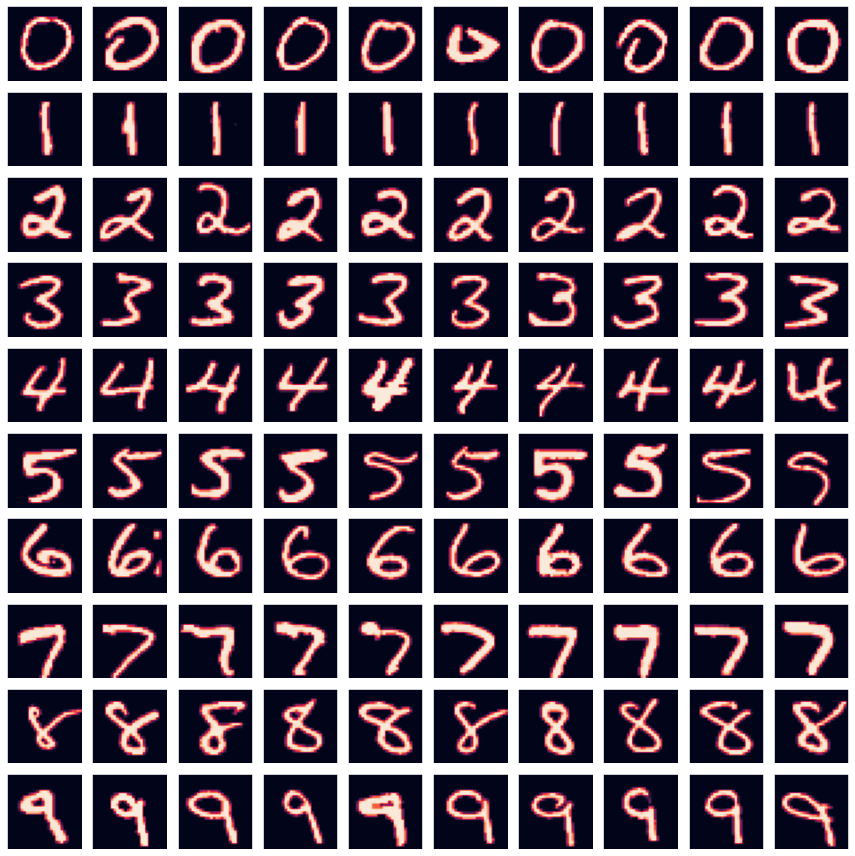
\includegraphics[scale=0.37, trim={0 0 425 0},
    clip]{mnist-far-from-boundary.png}\label{subfig:far}} 
    
    \caption{After finding out the adversarial paths from each training point to
    the decision boundary of a model trained on MNIST, we visualized some points
    closest to and farthest from the decision boundary. Examples pertaining to
    each class have been put on different rows: 0 to 9 from top to bottom. Note
    that the path to the next class was found by
    untargeted-unbounded-gradient-ascent, which is why label noise is such that
    some of the 0s look like 1s, 1s like 2s, and so on. Constratingly, the
    images on the right are far away from the boundary, again evaluated in a
    targeted manner. These images seem very crisp.}
    \label{fig:pgd-path-examples}
\end{figure}

% write an algorithm for the targeted version
% write an algorithm for the untargeted version

\subsection{Using adversarial paths to analyse poisons}

For a given dataset, we first train a classifier on the clean datasets, without
placing any mislabeled poisons. Let us call this the \emph{clean classifier}. We
then iterate over the training set, and find out adversarial paths for each
point.

The hypothesis is that if points are too close to the decision boundary, then it
is not very optimal to mislabel them (optimal in the sense that the adversarial
\emph{error} of a model trained on the dataset with mislabeled points has to be
maximal), since the decision boundary is going to slightly be modified to
accommodate the poison. If it is too far away, then it might be the case that
the classifier resorts to memorising the poison using an alternative pocket,
rather than modify the natural decision boundary.

\begin{algorithm}[!h]
\caption{Targeted Unbounded Gradient Ascent}
\begin{algorithmic}[1]
\Procedure{Adversarial-Path}{$\mathcal{C}, \vec{x}, t, m, \epsilon$}
    \State Path $\gets [\vec{x}]$
    \State Output $\gets \mathcal{C}(\vec{x})$
    \While{len(Path) $\leq m$ and $t \neq$ Output}
        \State $\vec{x} =$ \textproc{Targeted-FGSM}($\mathcal{C}, \vec{x}, t, \epsilon$)
        \State Path.append($\vec{x}$)
        \State Output $\gets \mathcal{C}(\vec{x})$
    \EndWhile
    \State \Return Path
    \label{algorithm:unbounded-gd}
\EndProcedure

\end{algorithmic}
\end{algorithm}


\subsection{The experiments}

\subsubsection{0-1 MNIST}
    We only consider a 2-class dataset, composed of the classes ``0" and ``1",
    from MNIST.

    A binary classifier is trained on this dataset. We then find out the
    adversarial paths for each point in the training set. Figure
    \ref{fig:0-1-mnist-pgd-path} shows an illustration of the distribution of
    the length of these paths over the training set points, per class.

    Next, we divide the training set points into various disjoint buckets, each
    bucket holding points from a different range of the length of the
    adversarial path. Essentially, the $x$-axis of \ref{fig:0-1-mnist-pgd-path}
    is divided into ranges, and points falling into each range are put into the
    bucket for that range.

    \begin{figure}[!h]
        \centering
        \subfloat[][Distribution of the length of adversarial paths, over each
        class of 0-1
        MNIST.]{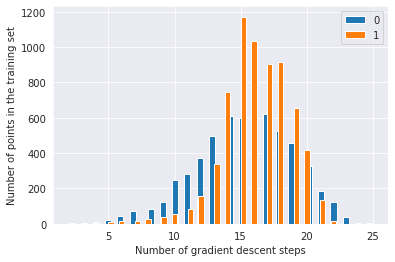
\includegraphics[scale=0.44]{0-1-MNIST-pgd-scores.png}}
        \qquad
        \subfloat[][Adversarial accuracy of network trained on a poisoned 0-1
        MNIST dataset, with poisons selected at increasing distances from the
        decision boundary.]{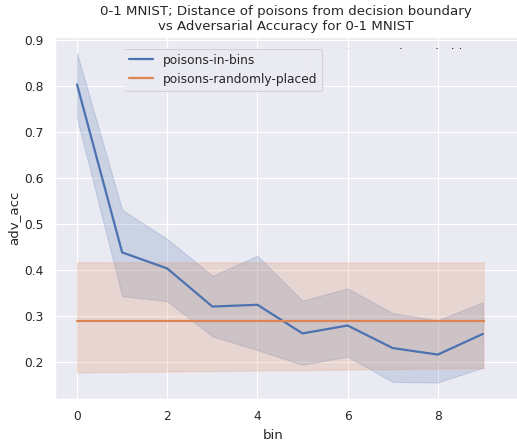
\includegraphics[scale=0.33, trim={0 0 0 33},
        clip]{0-1-MNIST-pgd-scored-curve}} \caption{(a) shows the distribution
        over the number of gradient ascent updates it took for the classifier to
        flip its output, for 0-1 MNIST, for the points in the training set. The
        $y$-axis indicates the number of points in the training set. The step
        size used for the above was 0.01, on $[0, 1]$ normalized input images.
        (b) The $x$ axis only denotes an ordinal value: higher values represent
        buckets holding points for which the adversarial paths were lengthier.
        The points were segregated into different buckets for (b), each bucket
        having points at a certain distance range from the boundary. The test
        accuracy of all of the above models are greater than 99\%.}
        \label{fig:0-1-mnist-pgd-path}
    \end{figure}

    We train several models for each bucket, each with randomly selected poisons
    from that bucket. Figure \ref{fig:0-1-mnist-pgd-path} illustrates the results.
    Closer the mislabeled points are to the original decision boundary, less the
    fall in the adversarial accuracy of the model trained after mislabeling that
    point. As we go farther from the decision boundary, the poisons have a
    greater impact. The next experiment will shed more light on placing poisons
    even farther from the boundary (in the full MNIST case, where some classes
    were observed to be even farther from the decision boundary), and the impact
    of the poisons starts wearing away.

    

\subsubsection{MNIST}
    We now consider the full MNIST dataset, and any points selected to be
    mislabeled, will be cyclically set to the next class in $[0..9]$. We first,
    like we did previously, find out the adversarial paths for each training
    point. But since we are flipping the label to the next class, we will find
    out adversarial paths for each point in a targeted manner, with the next
    class being the target.

    Figure \ref{fig:full-mnist-pgd-path} shows the distribution of the number of
    gradient descent steps each adversarial path took, i.e. the length of the
    targeted-adversarial paths for each point in the training set. First of all,
    we observe that we cannot have universal buckets for all classes, since some
    classes are much farther from the decision boundary than others. For
    instance, points in class 1 are much closer to the boundary than points in
    class 9. So it is not possible to do experiments where we flip points in the
    same range for all classes. There is a solution however, which is that we
    only place mislabeled poisons for \emph{one class} of the dataset, flipping
    the label cyclically to the next class. The adversarial accuracy of the
    resultant network will only be evaluated on targeted attacks from that
    selected class, to the next one (the class the labels were flipped to).

    The results of this experiment show that the closer the mislabeled points
    are to the decision boundary, lower their impact. As we mislabel points
    farther from the boundary, the impact increases, until a certain point.
    After a point, selecting points farther from the decision boundary worsens
    the impact. The curves are as shown in figure \ref{fig:full-MNIST-curve},
    and the 3 graphs shown are for classes 1, 4, and 9 flipped to 2, 5, and 0
    respectively. These classes were chosen since they are at increasing
    distances from the decision boundary. Points in class 1 are very close, and
    points in class 9 are very far. So they capture cases at different regions
    in the spectrum.

    Also, the minima observed for all the curves is where most of the training
    set points lie, which explains why the random strategy manages to cause a
    huge fall in the adversarial accuracy. Randomly selecting points to flip
    still has a high chance of selecting these impactful points, since there are
    so many of them.

    \begin{figure}[!h]
        \centering
        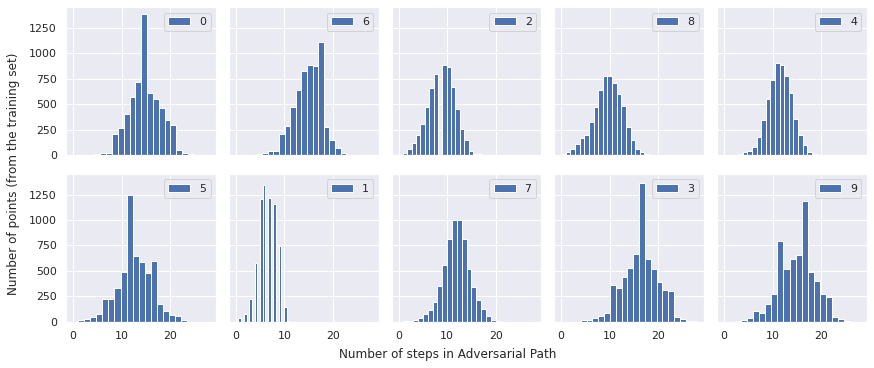
\includegraphics[scale=0.425]{full-MNIST-pgd-scores.png}
        \caption{Distribution over the number of gradient ascent updates it took
        for the classifier to flip its output, for the full MNIST dataset, for
        the points in the training set. The $y$-axis indicates the number of
        points in the training set. The step size used for the above was 0.01,
        on $[0, 1]$ normalized input images. Note that for training points
        belonging to class ``1", it takes not more than 10 steps in these
        adversarial paths. This means that for an attack radius of
        $\epsilon=0.1$, almost the entire class must be vulnerable, which is
        indeed the case. The adversarial accuracy of the model trained on the
        clean dataset, on targeted attacks from 1 to 2 is 0.}
        \label{fig:full-mnist-pgd-path}
    \end{figure}

    % insert impact figure(s) here
    % need to generate other figures

    \begin{figure}[!h]
        \centering
        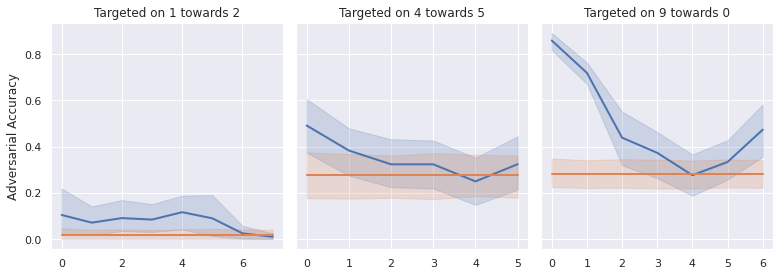
\includegraphics[scale=0.5]{targeted-mnist-pgd-path-trick.png}
        \caption{Full MNIST dataset. The $x$ axis only denotes an ordinal value:
        higher values represents represents buckets holding points for which the
        adversarial paths were lengthier. The orange line is a baseline showing
        the adversarial accuracy when same number of points are randomly
        selected to poison. The 3 graphs shown are for classes 1, 4, and 9
        flipped to 2, 5, and 0 respectively. These classes are at increasing
        distances from the decision boundary: points in class 1 are very close,
        and points in class 9 are very far, class 4 being an intermediate case.
        The adversarial accuracy evaluation for each case is done using targeted
        attacks from classes 1, 4, and 9 to 2, 5, 0 respectively to study the
        effects of poisons. 10 poisons were placed per class for these runs. The
        test accuracy of all of the networks evaluated in the above diagram is
        more than 99\%.}
        \label{fig:full-MNIST-curve}
    \end{figure}


This provides a way to select points to flip, given a budget. We can fit a clean
model to the dataset, and find out adversarial paths for each point. The
targeted or untargeted nature of the adversarial path will depend on the kind of
vulnerabity we want in the victim's model. For instance, if we decide to flip a
class $A$ to a class $B$, then the adversarial paths should be targeted from $A$
to $B$, after which the victim's model will be vulnerable to targeted attacks
from class $A$ to class $B$. We can then perform an analysis over the different
adversarial path lengths, fitting models for each case, which will guide towards
refining our search towards a smaller set of points to search over.

\chapter{Future Work: A Meta-Learning Approach}
The problem of \emph{crafting} label noise can be framed as a multi-level
optimisation problem. While meta-learning is a broadly used term, we will be
referring to the \emph{gradient-based} meta-learning setup
\citep{maml,first-order-meta,forward-reverse-hyperparameter}. Under this setup,
we have an inner objective, $\mathcal{L}^\text{in}$ minimised inside a loop, and
outer objective $\mathcal{L}^\text{out}$, minimised in an outer-loop, nesting
the inner objective inside of it. There are certain parameters $\phi$ utilised
by the training setup of the inner loop, which the outer loop has control over,
and parameters $\theta$ which the inner loop has control over. The aim is to
compute gradients $\nabla_\phi \mathcal{L}^\text{out}$ to make gradient-descent
updates to $\phi$. The way this gradient computation is done, is by unfolding
training steps in the inner loop, and backpropagating through the gradient
updates made in this inner loop.

For simplicity, let us assume we have to solve a binary classification problem.
There are only $2$ classes, and we are given a dataset with $n$ points sampled
from $\mathcal{P}$, and labeled with the ground truth labeling function $c$ to
produce a dataset $S_{\text{clean}}=\{(\vec{x}_i, c(\vec{x}_i))\}_{i=1}^n$. 

We are to find one point in this dataset, i.e. some $i \in \{1..n\}$. This point
should be such that if the given point's label is flipped to the other class,
the adversarial accuracy of a classifier trained on this modified, or
\emph{poisoned} dataset is as low as possible.

The following are different agents optimising over different variables in the
problem we are concerned with:
\begin{enumerate}
    \item The \emph{victim} optimises over the model parameters, attempting to
    minimise the training loss
    \item The \emph{input adversary}, as we will call it, optimises over
    constrained perturbations to the input, attempting to maximise the training
    loss
    \item The \emph{poisoning adversary}, as we will call it, optimises over
    which points to carry out a label change, given a budget constraint over the
    number of labels it can modify, and attempts to minimise the adversarial
    accuracy of the model
\end{enumerate}
Note that in each case, the agents are concerned with maximising or minimising
\emph{accuracy}, but the loss is the only metric under control. An appropriate
loss, when minimised or maximised, can be expected to increase/decrease the
accuracy of the model.

Let the size of the training set be $n$. Let the label noise the poisoning
adversary adds to the training set be represented as $\vec{\Delta y} \in \{0,
1\}^{n}$ such that $\sum_i \vec{\Delta y}_i = 1$, $\vec{y}$ being the vector of
labels in the dataset, $i$th label being $\vec{y}_i$, $X$ being a matrix storing
the training points as its row vectors, with the $i$th data point being
$\vec{x_i}$. Let $\mathcal{H}$ be the hypothesis class, i.e. the set of
functions the \emph{victim} is optimising over (one example of a hypothesis
class is the set of all neural networks of a fixed architecture, with different
parameter values). The problem can then be framed as:
\begin{equation}
    \label{eq:optimization}
    \begin{split}
    \vec{\Delta y}^*
    =
    {\underset{\vec{\Delta y}~\text{is one-hot}}
    {\arg\max}}~
    \mathcal{R}_{\text{Adv}}^{\rho}
    \biggl (
        \underset{\mathcal{C} \in \mathcal{H}}{\arg\min}~
        \mathcal{L}(\mathcal{C}, X, \vec{y} \oplus \vec{\Delta y})
    \biggr )
    \end{split}
\end{equation}
where $\oplus$ is the ``xor" operation, i.e. allows label flipping to happen
wherever $\vec{\Delta y}$ is one-hot at. This can be practically implemented as
\begin{equation}
    \label{eq:optimization-prac}
    \begin{split}
    \vec{\Delta y}^*
    =
    {\underset{\vec{\Delta y}~\text{is one-hot}}
    {\arg\max}}~
    \underset{X' \in \mathcal{B}_\rho^{p}(X)}{\max}~\mathcal{L} \biggl(
    \underset{\mathcal{C} \in \mathcal{H}}{\arg\min}~
    \mathcal{L}(\mathcal{C}, X, \vec{y} \oplus \vec{\Delta y}),
    X', \vec{y}
    \biggr)
    \end{split}
\end{equation}
where $\mathcal{B}_\rho^{p}(X)$ is defined as the set of all matrices $M$ such
that $\forall i \in \{1..n\}$, $\vec{m_i} \in \mathcal{B}_\rho^{p}(\vec{x_i})$.


While implementing, we can have a learnable real valued vector $\vec{h}$ with
dimensionality $n$ where $n$ is the training set size. Let us call this the
\emph{flip logit vector}. We derive a one-hot vector over the training set using
$\vec{h}$, by using the Gumbel-Softmax trick used to create a ``smooth" function
that behaves like argmax, but that allows gradients to backpropagate
\citep{DBLP:conf/iclr/MaddisonMT17}. Given a logit vector $\vec{h}$, the
Gumbel-Softmax trick produces the almost one-hot vector $\vec{f}$ such that:
\begin{equation*}
    \vec{f}_i = \frac{\exp((\vec{h}_i + \vec{g}_i)/\tau)}
        {\sum_{j=1}^n \exp((\vec{h}_j + \vec{g}_j)/\tau)}
\end{equation*}
where $\tau > 0$ is a hyperparameter called the temperature and $\vec{g}$ is an
$n$-dimensional vector such that each entry of it, $\vec{g}_i$ is sampled from
the  Gumbel Distribution i.i.d.

Now that we have $\vec{f}$, such that we can backpropagate gradients through it,
we show the model we are training on (we do not need the exact same model that
the \emph{victim} might be using. Most attacks in literature which make use of
models to craft the attack assume a model and hope that the attack generalizes,
which works very well practically) the modified label vector
\begin{equation*}
    \vec{y'} = \textbf{y}\odot(1-\textbf{f})+\textbf{y}\odot(1-\textbf{f})
\end{equation*}
Now we make gradient updates on the network we have, simulating training with
these new labels, and recording all operations we do, use the final network
produced by these updates to craft adversarial examples from the training set
itself, and finally computing the loss of this final model on the adversarial
examples. This loss has to be \emph{maximised}. So we backpropagate from this
loss, and receive gradients for $\vec{h}$ through $\vec{f}$, and we do a
\emph{gradient ascent} on $\vec{h}$.

We could not find a computationally feasible way to implement this. Practical
datasets have thousands of training examples per class, and the inner loop of
this method involves multiple gradient descent steps, which means we will have
to calculate and backpropagate second order gradients through these steps, while
involving the entire training set in the update steps, so as to get gradients
back to each dimension of $\vec{f}$, since we require exactly one dimension
selected by $\vec{f}$. Further, after the updates in the inner loop, we also
need to compute adversarial examples for each point in the training set, with
the final updated network, and the outer loop's maximisation is done over these
adversarial examples. Figure \ref{fig:bilevel-opt} shows an example for a small
dataset with just 2 batches of size 4.

% \pagebreak[4]
%   \global\pdfpageattr\expandafter{\the\pdfpageattr/Rotate 90}
\begin{figure}
    \centering
    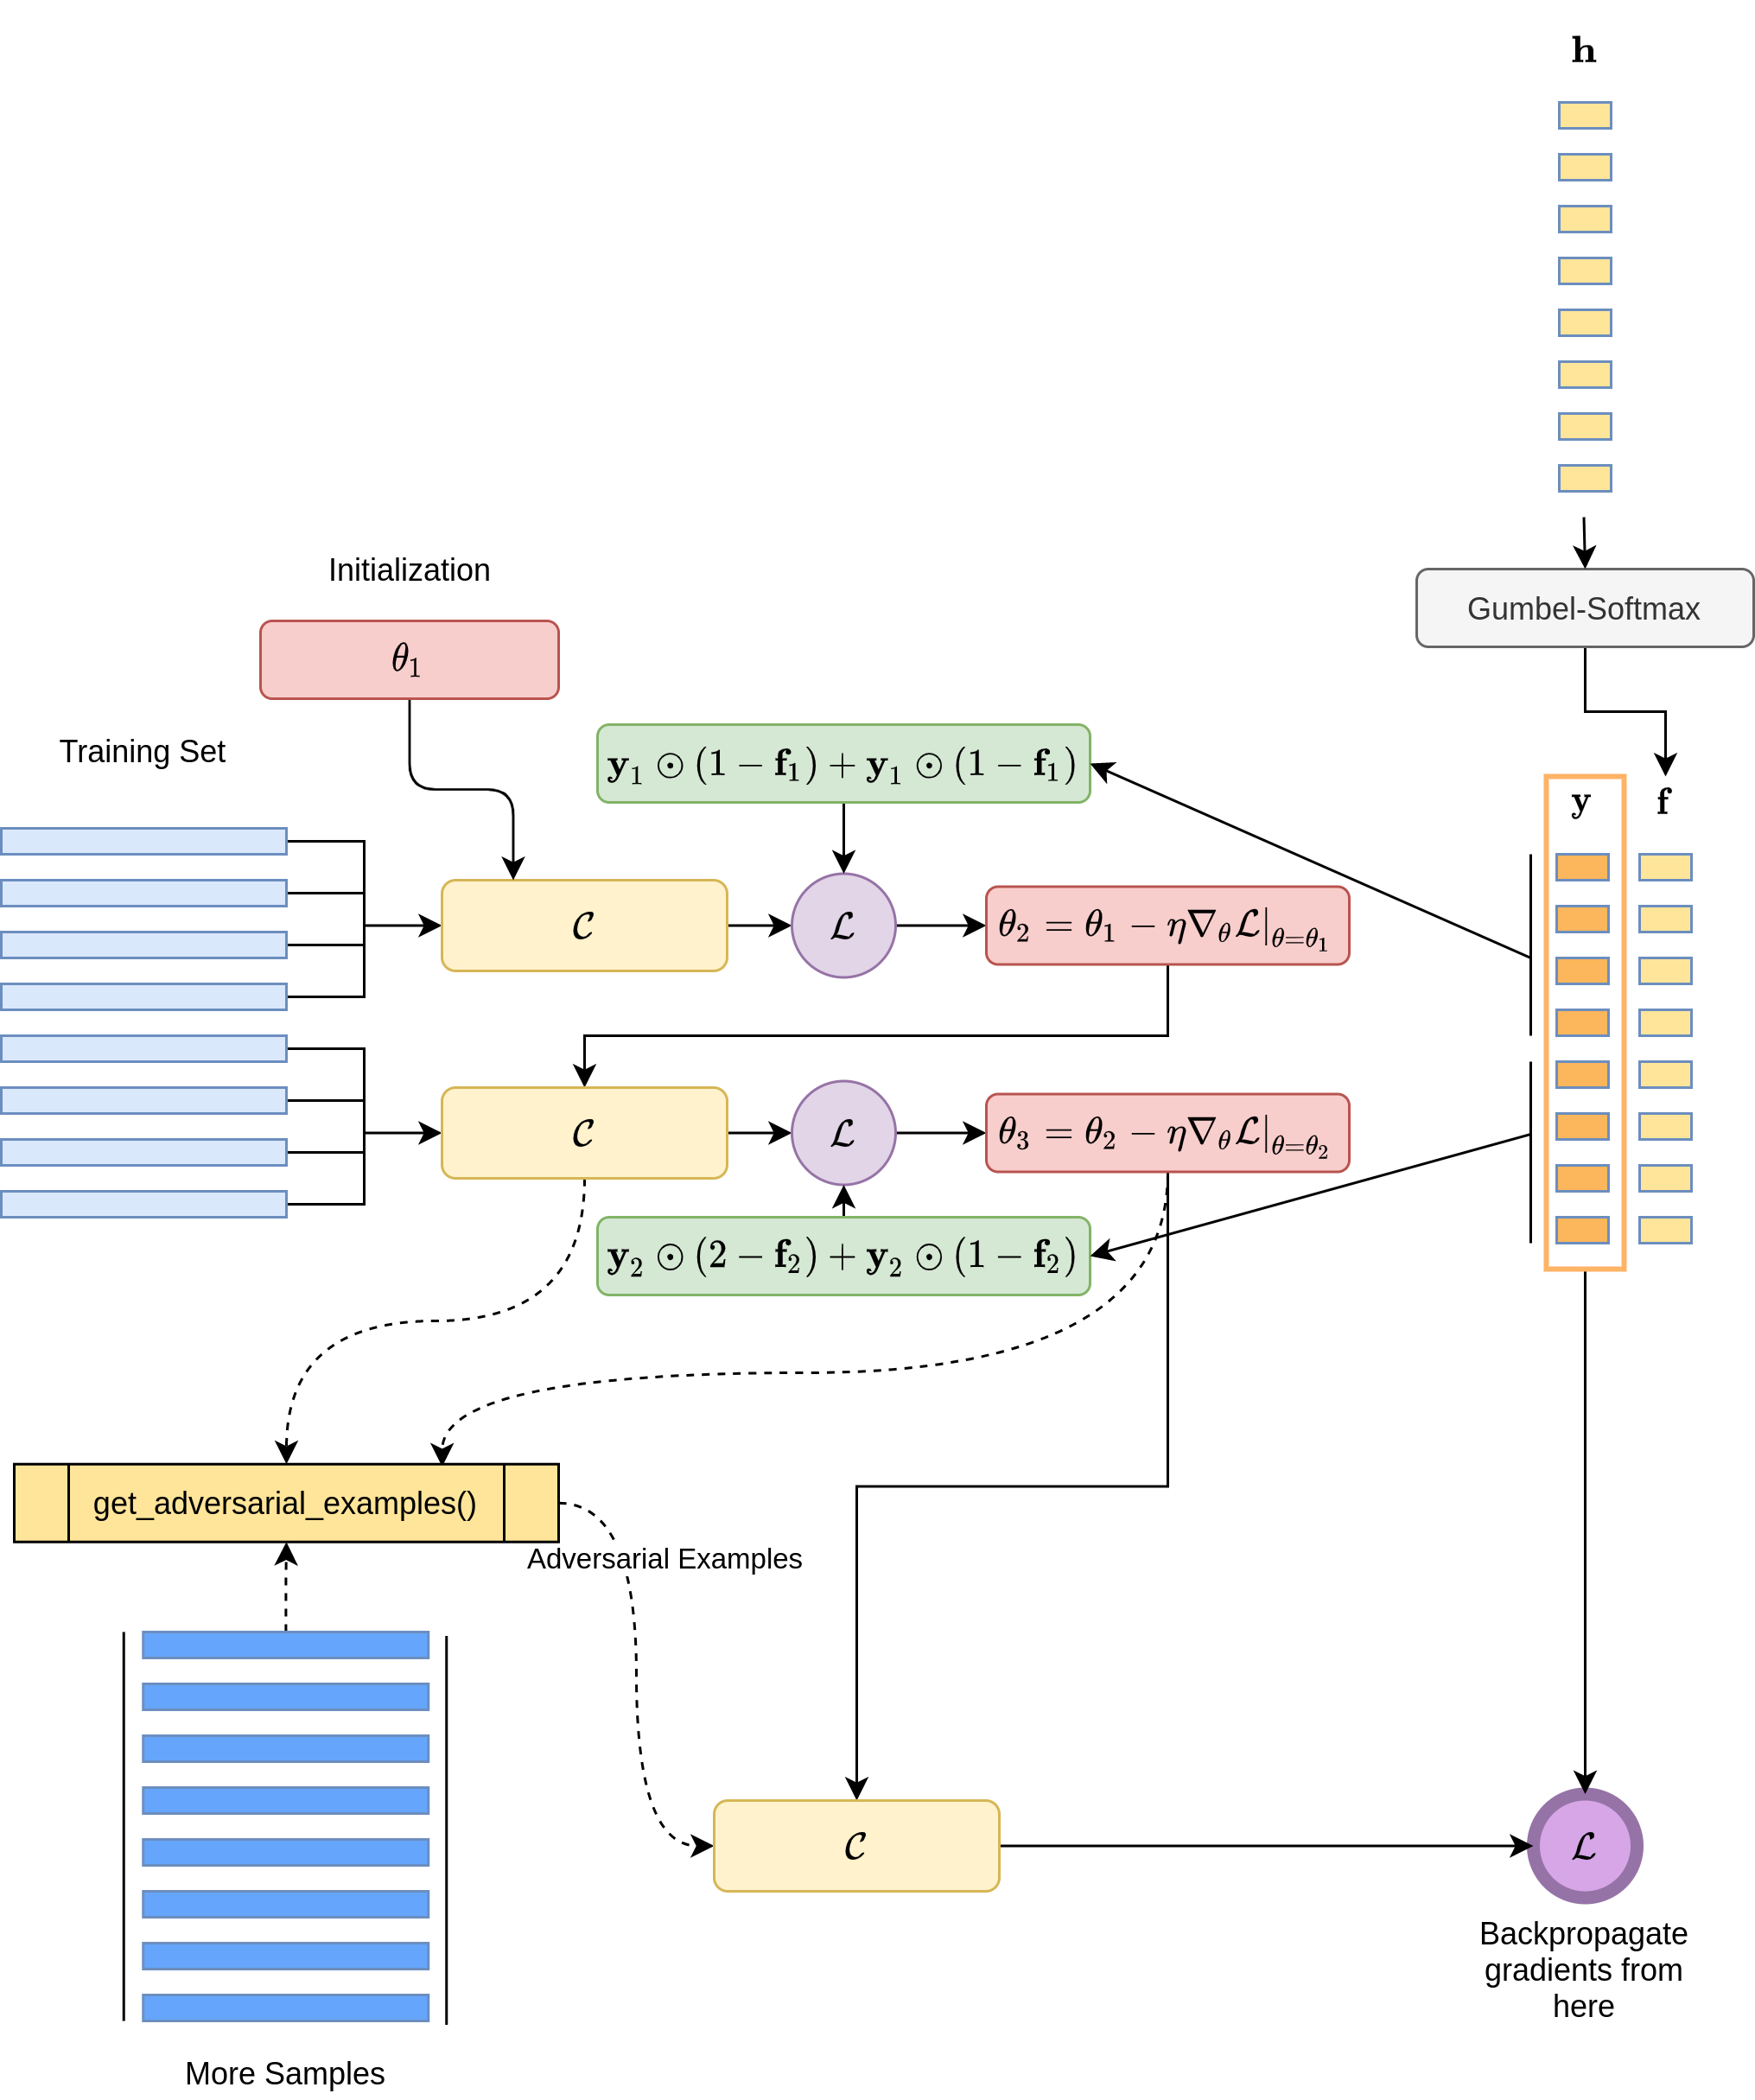
\includegraphics[scale=0.17]{biplot.png}
    \caption{An example of the multi-level optimisation case, where we have a
    small dataset of 8 examples, and two gradient updates are made in the
    innermost loop, with each batch update having 4 examples. The function
    get\_adversarial\_examples () produces adversarial exapmles for a given
    network and inputs. Dotted lines indicate that the operations are not to be
    recorded, and bold lines indicate that the operations should be recorded, so
    that we can pass gradients through them during the backward pass. $\odot$
    refers to elementwise multiplication.}
    \label{fig:bilevel-opt}
\end{figure}

\chapter{Conclusion}
The ideas discussed in this thesis uncover properties of neural networks as they
memorise label noise. We establish that placing mislabeled points at the highest
probability density regions is sub-optimal to hurt the adversarial accuracy of
models, and also provide a way to select points to label flip, by analysing
their adversarial paths for models trained on clean data.

While we extend and also provide a new bound for the adversarial risk, when
classifiers memorise label noise, it is clear from the experiments in this
thesis that these bounds, as well as the one in literature, with regards to
uniform label noise are highly vacuous in practice. This is because networks
seem to be much more smoother in memorising poisons than these analyses assume.
The regions wrongly learnt by networks are much larger in size, rendering a
large amount of probability mass vulnerable.

The adversarial path experiments conducted show that the points that hurt the
adversarial accuracy the most when mislabeled, are the ones which force the
network to learn complex decision boundaries. If in order to memorise a
mislabeled point, networks tweak the decision boundary they would have learnt
otherwise, in the absence of that mislabeled point, the adversarial accuracy is
massively hurt. These ideas could be used to carefully select points to
label-flip in a dataset, given budget constraints. By analysing the adversarial
paths of training points, on a model trained on the clean dataset, we can select
points that are best to poison.


\clearpage
\bibliographystyle{plainnat}
\bibliography{ref}
\end{document}
